\section{光の粒子性・物質波と原子模型}

% ===========================================================================
%  再編（2026-09-24）：第5章 原子物理 の第33回（原子の初回）．
%  原本の 第42回「光電効果(1)」・第43回「光電効果(2)・コンプトン効果」・第44回「水素原子モデル」の全体と，
%  第45回の 45.1「水素原子の発光スペクトル」を1回にまとめた（45.2 以降は第34回）．
%
%  ・章扉 `{\Huge \bf 第5章　原子物理}` は落とした（physics_new14〜32.tex と同じ）．
%
%  ・練習は9題．原子物理の練習番号は章の先頭から［1］〜と数える（\setcounter{qno}{0}）．
%      ［1］＝A問題の統合（㊷[1]＋㊸[4]＋㊹[8]．設問は10個とも残した）
%      ［2］＝㊷[2]（ミリカンの実験・指定）  ［3］＝㊷[3]（光電効果・指定）
%      ［4］＝㊸[5]（光電管・指定）  ［5］＝㊸[6]（コンプトン効果・指定）
%      ［6］＝㊹[9]（ボーアモデル・指定）  ［7］＝㊺[11]（水素原子のスペクトル・指定）
%      C問題 ［8］＝㊸[7]（光電管とコンデンサー）  ［9］＝㊹[10]（フランク・ヘルツの実験）
%    再編案の表は第33回を「10題」としているが，㊷[1]〜㊺[11] の11題から A問題3→1 で2題減るので9題が正しい
%    （原子全体では 25−1（[23]は第29回へ）−2＝22題で，第34回が13題）．
%
%  ・例題は7題．原子物理（原本 第5章）の例題は章の先頭から1・2・3…と数えるので【例題1】〜【例題7】
%    （\setcounter{nombre}{0}）．原本の例題1〜7 をそのまま使った．理想の4題より多いが，
%    いずれも小問1〜2個の短い確認問題で，原本の節ごとに1題ずつ付いているので削らなかった．
%
%  ・【重要】原本の講義編（例題を含む）は Google Drive の OCR テキストしか取れなかった．
%    本文は physics_ch42〜45.tex の打ち込みを使い，例題の問題文は OCR から復元した．要照合：
%      ・例題1：データ 6.43・9.69・12.89・11.28・8.05（×10^{-19} C）は OCR の通り（4〜8倍になり整合）．
%      ・例題3：(1) は「500 nm 以上の波長で光電子を出さない光電管に 400 nm の光」までは読めたが，
%        問うている量（最大の速さか運動エネルギーか）が読めない．「最大の速さ」とした．
%        (2) のグラフは OCR に曲線の区別（a・b・c）と $-V_{\mathrm{a}}$ 程度しか残っておらず，**グラフは再構成**した．
%      ・例題4：図・記号（散乱角 θ，電子の角 φ）は再構成．設問 (1)(2)(3) は OCR の通り．
%      ・例題7：振動数 ① 4.57×10^{14} Hz，② 7.32×10^{14} Hz（OCR の「7.3210」を 7.32×10^{14} と読んだ．
%        n=6→2 の遷移 3.02 eV に一致）．(2) は OCR では「②は何系列か」だが，①②とも問う形にした．
%
%  ・原本の本文の誤り・欠落を直した：
%      (a) 44.2 の「光子を吸収して電子がよりエネルギーの低い準位に移動することを放射」は打ち込みの脱落．
%          OCR により「光子を吸収して高い準位に移ることを励起，光子を放出して低い準位に移ることを放射」に．
%      (b) 44.2 の $e_n$，$\dot n^2$ は $E_n$，$n^2$ の誤植．42.1 の「粘性係数は $6\pi\eta rv_1$」は粘性抵抗．
%      (c) 解答の誤り：㊹[10] の指針「$E_2-E_1=4.9$ [J]」→ eV．
%      (d) 旧回の番号による参照（「テキストの例題」など）を例題番号に付け替えた．
%
%  ・原本の本文に無く，練習が前提にしていたものを加筆した：
%      ・33.4 の後に{光の二重性}のまとめ（粒子性を示す現象／波動性を示す現象．練習［1］(7)，［3］）．
%      ・33.7 に{電子の衝突による励起}（フランク・ヘルツの実験の前提．弾性衝突・非弾性衝突の言葉）．
%      ・33.8 に{リュードベリの式}と{リュードベリ定数}（練習［7］の前提．原本は問題文で初めて出てくる）．
%
%  ・図：講義の図は講義編から切り出し済みのもの（img/text/text2_p94〜p107）．
%    練習・解答の図は `mkfig_new33.py`＋`jobs_new33.py`，例題の図は `mkfig_new33ex.py`（TikZ 自作）．
% ===========================================================================

% 空欄と選択肢（この回と第34回で使う）
\def\BOX#1{\framebox[4zw]{\rule{0pt}{1.1zw}#1}}
\def\Sentaku#1{{\small\{選択肢：#1\}}}

% 例題番号：原子物理（原本 第5章）の例題は章の先頭から1・2・3…
\setcounter{nombre}{0}

\subsection{ミリカンの実験}

ミリカンは，帯電させた油滴を電場をかけた空気中で上下運動させることによって，電気素量$e$の値を決定することに成功した．

\begin{center}

\includegraphics[keepaspectratio,width=110mm]{text2_p94_fig1.png}
\end{center}

上図はその実験装置である．
油を霧吹きで拡散して霧状にすると，その一部が小さい穴を通して下の部屋へと落ちてくる．
下の部屋には軽くX線が照射されて空気が少し電離しており，このイオンに触れた油滴は帯電する．
この油滴には重力と空気の粘性抵抗が作用するため，これらの力がつり合って一定の速度で落下する．
油滴の半径を$r\U{m}$，密度を$\rho\U{kg/m^3}$，一定となったときの速さを$v_1\U{m/s}$，空気の粘性係数を$\eta\U{kg/(m\cdot s)}$とすると，油滴の質量は$\dfrac{4}{3}\pi\rho r^3\U{kg}$，粘性抵抗は$6\pi\eta rv_1\U{N}$で与えられることが知られているので，つり合いの式は
\[\frac{4}{3}\pi\rho r^3g=6\pi\eta rv_1\]
となる．

次に，下の部屋に下向きに強さ$E\U{N/C}$の電場をかけると，負に帯電した油滴は電場から上向きの力を受け，今度は上向きに運動させることができる．
上向きに運動するようになると粘性抵抗は下向きに作用するようになり，力がつり合って一定の速さで上昇するようになる．
油滴の帯電量を$-q\U{C}$，一定となったときの上昇の速さを$v_2\U{m/s}$とすると，力のつり合いの式は
\[\frac{4}{3}\pi\rho r^3g+6\pi\eta rv_2=qE\]
となる．これら2つの式から測定が難しい$r$を消去して$q$を求めれば
\[q=\frac{9\pi(v_1+v_2)}{E}\sqrt{\frac{2\eta^3v_1}{\rho g}}\U{C}\]
となり，この式から油滴の電荷が計算される．
こうして油滴の電荷を実際に測定したところ，{\gtfamily 電荷は必ずある一定値の整数倍になっている}ことが分かった．このことから，電気素量が
\[e\fallingdotseq 1.60\times 10^{-19}\U{C}\]
であることが実験的に得られた．

%%%%%%%%%%  例題1（原本の【例題1】）  %%%%%%%%%%%%%%%%%%%%
\bsNeed{50mm}
\begin{reidaiunit}
\begin{reidai}{ミリカンの実験}
\hspace{1zw}ある油についてミリカンの実験を行い，その電荷を測定したところ，以下のような結果が得られた．
\[\text{\MARU{1}}\ 6.43,\quad\text{\MARU{2}}\ 9.69,\quad\text{\MARU{3}}\ 12.89,\quad\text{\MARU{4}}\ 11.28,\quad\text{\MARU{5}}\ 8.05\qquad(\text{単位は}\ 10^{-19}\U{C})\]
この実験結果を元にして，電気素量を有効数字3桁で求めよ．
\end{reidai}

\begin{sisinE}
電気素量の値がどの程度であるかは分からないので，まず電気量のおおざっぱな値を知るところから始める．\MARU{1}〜\MARU{5}の値がある特定の値の整数倍になっているのであれば，その差も必ずその特定の値の整数倍になる．そこで
(i)\ 実験結果を小さい方から順に並べて差を取り，おおざっぱな電気素量を求める．
(ii)\ \MARU{1}〜\MARU{5}が電気素量何個分に相当するかを考えて，その後平均を取って電気素量を求める．
\end{sisinE}

\Key{電荷の差を取っておおざっぱな$e$ \ $\Rightarrow$\ 各電荷が$e$の何倍か \ $\Rightarrow$\ 合計どうしの比で平均}

\begin{kaitou}
小さい方から並べると$6.43$，$8.05$，$9.69$，$11.28$，$12.89$（$\times 10^{-19}\U{C}$）で，その差は$1.62$，$1.64$，$1.59$，$1.61$である．よって電気素量はおよそ$1.6\times 10^{-19}\U{C}$と考えられ，\MARU{1}〜\MARU{5}はそれぞれ$4e$，$6e$，$8e$，$7e$，$5e$に相当する．以上より
\[e=\frac{6.43+9.69+12.89+11.28+8.05}{4+6+8+7+5}\times 10^{-19}=\frac{48.34}{30}\times 10^{-19}\fallingdotseq 1.61\times 10^{-19}\U{C}\Ans\]
\end{kaitou}
\end{reidaiunit}

\subsection{光電効果}

\begin{zuright}{44mm}
\hspace{1zw}金属に比較的波長の短い電磁波（光や紫外線など）を照射すると，金属表面から電子が飛び出す．
この現象を{\gtfamily 光電効果}といい，飛び出した電子のことを{\gtfamily 光電子}と呼ぶ．
この現象を調べるうちに，以下のような特徴があることが分かった．
\zusep

\includegraphics[keepaspectratio,width=40mm]{text2_p95_fig1.png}
\end{zuright}

\bsNeed{40mm}
\begin{matome}{光電効果の特徴}
\begin{description}
\item[\MARU{1}] 当てる光の振動数$\nu\U{Hz}$（ニュー）が，金属の種類に固有な値（{\gtfamily 限界振動数}$\nu_0$）より小さい場合には，どんなに光量が多くても（光が強くても）電子は出ない．
\item[\MARU{2}] 逆に，$\nu>\nu_0$のときには光量が少なくても，ただちに電子が放出される．
\item[\MARU{3}] 飛び出す電子の運動エネルギーの大きさはさまざまな値をとるが，その{\gtfamily 最大値$K_{\max}$は振動数$\nu$に対して一意的に決まる}．
\item[\MARU{4}] 当てる光の振動数$\nu$を大きくしていくと，$K_{\max}$は大きくなる．
\item[\MARU{5}] $\nu$が一定のときは，光量を多くしても$K_{\max}$は変化しない．
\end{description}
\end{matome}

\begin{zuright}{48mm}
\hspace{1zw}金属内にある自由電子は金属イオンから引力を受けて束縛されている．
そのため，金属内から自由電子を飛び出させるためには，この引力を振り切るだけの仕事（エネルギー）を与えてやる必要がある．
このエネルギーの最小値をその金属の{\gtfamily 仕事関数}$W$という．
金属表面から電子を取り出す場合と，金属内部から電子を取り出す場合とでは必要なエネルギーが異なるので，{\gtfamily 金属表面から電子を飛び出させるのに必要なエネルギーを仕事関数$W$とする}．
\zusep

\includegraphics[keepaspectratio,width=46mm]{text2_p95_fig2.png}
\end{zuright}

さて，\MARU{1}〜\MARU{5}の現象は，光を波動だと考えるとうまく説明することはできない．
波動のエネルギーはその振幅$A$の2乗，振動数$\nu$の2乗に比例するので，$\nu<\nu_0$であっても光の強さ，すなわち振幅$A$を大きくすれば電子は仕事関数$W$分のエネルギーをもらって飛び出すことができるはずである．

そこでアインシュタインは，{\gtfamily 光を，振動数に比例するエネルギーを持つ粒のようなもの（これを光子（光量子）と呼ぶ）だと考える}ことにより，この光電効果を説明することに成功した．

\bsNeed{34mm}
\begin{matome}{光量子説}
 \hspace{3mm} 振動数$\nu\U{Hz}$，波長$\lambda\U{m}$の光は，1個あたり
 \hspace*{8mm}\AnaB{$E=h\nu=\dfrac{hc}{\lambda}$}$\U{J}$ のエネルギー，\quad \AnaB{$p=\dfrac{h\nu}{c}=\dfrac{h}{\lambda}$}$\U{kg\cdot m/s}$ の運動量\\
 \hspace{3mm} を持つ光子の流れである．$h$は{\gtfamily プランク定数}と呼ばれる比例定数で，$h\fallingdotseq 6.63\times 10^{-34}\U{J\cdot s}$
\end{matome}

このように考えると，光電効果の特徴\MARU{1}〜\MARU{5}は，次のように説明できる．
\begin{description}
\item[\MARU{1}] エネルギーは，{\gtfamily 光子1個と電子1個との間でやりとりされる}（2個の光子が同時に1個の電子に作用する確率は極めて小さい）．$h\nu<W$となる振動数$\nu$ではどんなにたくさん光子があっても，1つ1つの光子の持つエネルギーは仕事関数$W$より小さいため，電子は金属の外に飛び出ることはできない．$W=h\nu_0$のようにおけば，$\nu<\nu_0$のときは電子は決して出ない．
\item[\MARU{2}] 逆に，$h\nu>W$，すなわち$\nu>\nu_0$であれば，光量（光子の数）が少なくてもただちに電子が放出される（ただし，光子が少なければ飛び出る電子も少なくなる）．
\item[\MARU{3}] 光電子の持つ運動エネルギーを$K$，電子を飛び出させるのに必要なエネルギーを$\Delta U$とすれば，エネルギー保存則より$h\nu=\Delta U+K$となるが，電子を金属のどこからたたき出すかによって$\Delta U$は変わるため，出てくる電子の運動エネルギーはさまざまな値をとる．$K$が最大値をとるのは$\Delta U$が最小のときで，それは電子を表面からたたき出すときである．このときの$\Delta U$が仕事関数$W$であるから，$h\nu=K_{\max}+W$となり，$K_{\max}$は光の振動数$\nu$に対して一意的に決まり，光量によらない．
\item[\MARU{4}] $h\nu=K_{\max}+W$の式から，$\nu$が大きくなれば明らかに$K_{\max}$も大きくなる．
\item[\MARU{5}] 光量を多くしてもエネルギーのやりとりは光子1個と電子1個の間で行われるから，光子がたくさんあっても$K_{\max}$は変わらない．
\end{description}

\bsNeed{24mm}
\begin{matome}{光電効果におけるエネルギー保存則}
 \hspace{3mm} 金属表面から電子が飛び出すときが最大運動エネルギーを持つときであり，\\
 \hspace{3mm} このとき\quad \AnaB{$h\nu=K_{\max}+W$}
\end{matome}

%%%%%%%%%%  例題2（原本の【例題2】）  %%%%%%%%%%%%%%%%%%%%
\bsNeed{50mm}
\begin{reidaiunit}
\begin{reidai}{光電効果}
\begin{komon}
\ko{1} 金属に振動数$\nu\U{Hz}$の光を当てると，$h\nu\U{J}$（$h$はプランク定数）のエネルギーを持った光子が金属中の電子と衝突し，金属表面から電子が飛び出す．ある金属にある波長の光を入射したところ，電子が飛び出してくることはなかった．電子が飛び出してくるようにするための行為として適切なものを，以下の\MARU{1}〜\MARU{3}の中から選べ．\\
\hspace*{1zw}\MARU{1}\ 入射する光の量を増やす\quad \MARU{2}\ 入射する光の波長を短くする\quad \MARU{3}\ 入射する光の波長を長くする
\ko{2} 仕事関数$W\U{J}$の金属に振動数$\nu\U{Hz}$の光を入射したとき，金属表面から電子が飛び出してきた．この電子の速さの最大値$v_{\max}\U{m/s}$を，$\nu$，$W$，プランク定数$h\U{J\cdot s}$，電子の質量$m\U{kg}$を用いて表せ．
\end{komon}
\end{reidai}

\begin{sisinE}
(1) 光子1個のエネルギー$h\nu=\dfrac{hc}{\lambda}$が仕事関数より大きくなければ電子は飛び出さない．光の量（光子の数）を増やしても，光子1個のエネルギーは変わらない．
(2) 表面から飛び出す電子の運動エネルギーが最大である．
\end{sisinE}

\Key{表面から電子が飛び出すときが最大エネルギーを持つ\ $\Rightarrow$\ $h\nu=K_{\max}+W$}

\begin{kaitou}
\begin{komon}
\ko{1} 光子1個のエネルギー$\dfrac{hc}{\lambda}$を大きくする必要があるので，波長を短くすればよい．\quad \MARU{2}\Ans
\ko{2} $h\nu=\dfrac{1}{2}mv_{\max}^2+W$より
       \[v_{\max}=\sqrt{\frac{2(h\nu-W)}{m}}\U{m/s}\Ans\]
\end{komon}
\end{kaitou}
\end{reidaiunit}

\subsection{光電管}

\begin{zuright}{56mm}
\hspace{1zw}実際に光電効果を起こし，電圧をかけて光電子を捕集して電流に変える装置が{\gtfamily 光電管}である．
この光電管に図のような回路をつなぎ，端子$\mathrm{D}$を動かすことにより，$\mathrm{A}$と$\mathrm{C}$の間にかける電圧を自由に変化させられるようにする．
光を図の金属板$\mathrm{C}$（受光板）に当てると，光子のエネルギー$h\nu$が金属の仕事関数$W$より大きい場合は光電子が放出されるが，この際に適当な電圧をかけると発生した光電子が$\mathrm{A}$（集電子板）に取り込まれ，これが電流として測定される．
この装置を用いると，光量や，飛び出た光電子の最大運動エネルギーなどを測定することができる．
\zusep

\includegraphics[keepaspectratio,width=54mm]{text2_p98_fig1.png}
\end{zuright}

\begin{zuright}{62mm}
\hspace{1zw}$\mathrm{A}$と$\mathrm{C}$の間にかける電圧を変えながらそのときに流れる電流を測定すると，右図のようなグラフが得られる．
このグラフを解釈するときは，電圧のかけ方により2通りに分けて考えるとよい．
\zusep

\includegraphics[keepaspectratio,width=60mm]{text2_p98_fig2.png}
\end{zuright}
\begin{description}
\item[\MARU{1}] {\gtfamily $\mathrm{C}$に対して$\mathrm{A}$の方が高電位になるように電圧をかける（$V_{\mathrm{AC}}>0$）}\par
$\mathrm{A}\to\mathrm{C}$向きに電場が生じるので，ある程度以上の電圧をかけるとこの電場によって$\mathrm{C}$を飛び出た電子を$\mathrm{A}$に集められる．生じた電子すべてが$\mathrm{A}$に集まるようになるとそれ以上は電流は増加しなくなる．そのため，{\gtfamily 飽和電流は$\mathrm{C}$で発生する光電子の数，すなわち$\mathrm{C}$に当たる光子の数（光量）によって決まる}．
\item[\MARU{2}] {\gtfamily $\mathrm{C}$に対して$\mathrm{A}$の方が低電位になるように電圧をかける（$V_{\mathrm{AC}}<0$）}\par
$\mathrm{C}\to\mathrm{A}$向きに電場が生じるので，$\mathrm{C}$を飛び出た電子は$\mathrm{C}$に押し戻されるような力を受ける．そのため，{\gtfamily ある一定以上の運動エネルギーを持った電子のみが$\mathrm{A}$に達する}．特に$V_{\mathrm{AC}}=-V$の電圧をかける場合，電子の位置エネルギーの差は$eV$であるから，$eV$以上の運動エネルギーを持った光電子のみが$\mathrm{A}$に達する．
\end{description}

\begin{zuright}{44mm}
\hspace{1zw}\MARU{2}の場合，さらに$V$を大きくしていき，$eV>K_{\max}$となると，もはやどの光電子も$\mathrm{A}$に達することができなくなる．
そのため，その限界の電圧$V$（これを{\gtfamily 阻止電圧}という）が分かれば，$K_{\max}=eV$から電子の最大運動エネルギーを計算することができる．
さまざまな振動数の光を用いて実験をすると，右のようなグラフが得られる．$h\nu=K_{\max}+W$より，グラフは傾き$h$，縦軸切片$-W$，横軸切片が限界振動数$\nu_0$の直線である．
\zusep

\includegraphics[keepaspectratio,width=42mm]{text2_p99_fig1.png}
\end{zuright}

\bsNeed{30mm}
\begin{matome}{光電管}
 \MARU{1}\ 受光板に対して集電子板を正電位にする\ $\Rightarrow$\ 電流は飽和する（飽和電流は\AnaB{光子の数}で決まる）\\
 \MARU{2}\ 受光板に対して集電子板を負電位にする\ $\Rightarrow$\ 電流は減少する（阻止電圧$V$から\AnaB{$K_{\max}=eV$}）
\end{matome}

なお，光電効果の現象を扱う際にはおおよそ$10^{-18}\sim 10^{-19}\U{J}$程度のエネルギーを扱うため，そのまま書くと指数が出てきて面倒である．
そこで，電子が$1\U{V}$の電位差により得られるエネルギーを$1\U{eV}$（{\gtfamily 電子ボルト}，エレクトロンボルト）と定義する．定義より
\[1\U{eV}=e\U{C}\times 1\U{V}\fallingdotseq 1.6\times 10^{-19}\U{J}\]
である．

%%%%%%%%%%  例題3（原本の【例題3】）  %%%%%%%%%%%%%%%%%%%%
\bsNeed{70mm}
\begin{reidaiunit}
\begin{reidai}{光電管}
\hspace{1zw}光電効果に関する以下の問題に答えよ．ただし，電気素量は$e=1.60\times 10^{-19}\U{C}$，プランク定数は$h=6.63\times 10^{-34}\U{J\cdot s}$，電子の質量は$9.11\times 10^{-31}\U{kg}$，光速は$c=3.00\times 10^8\U{m/s}$である．
\begin{zuright}{54mm}
\begin{komon}
\ko{1} $500\U{nm}$以上の波長の光では光電子を出さない光電管がある．この光電管の受光板に波長$400\U{nm}$の光を当てたときに飛び出す電子の速さの最大値を求めよ．
\ko{2} 光電管にかける電圧，光量，振動数などをいくつか選んで，そのときに流れる電流を測定したところ，図のようなグラフ$\mathrm{a}$，$\mathrm{b}$，$\mathrm{c}$を得た．このグラフの横軸は，\MARU{1}\ 集電子板に対する受光板の電位，\MARU{2}\ 受光板に対する集電子板の電位，のいずれか．また，$\mathrm{a}$，$\mathrm{b}$，$\mathrm{c}$の場合の光の振動数の大小関係，および光子数の大小関係をそれぞれ不等号（等号）を用いて表せ．
\end{komon}
\zusep
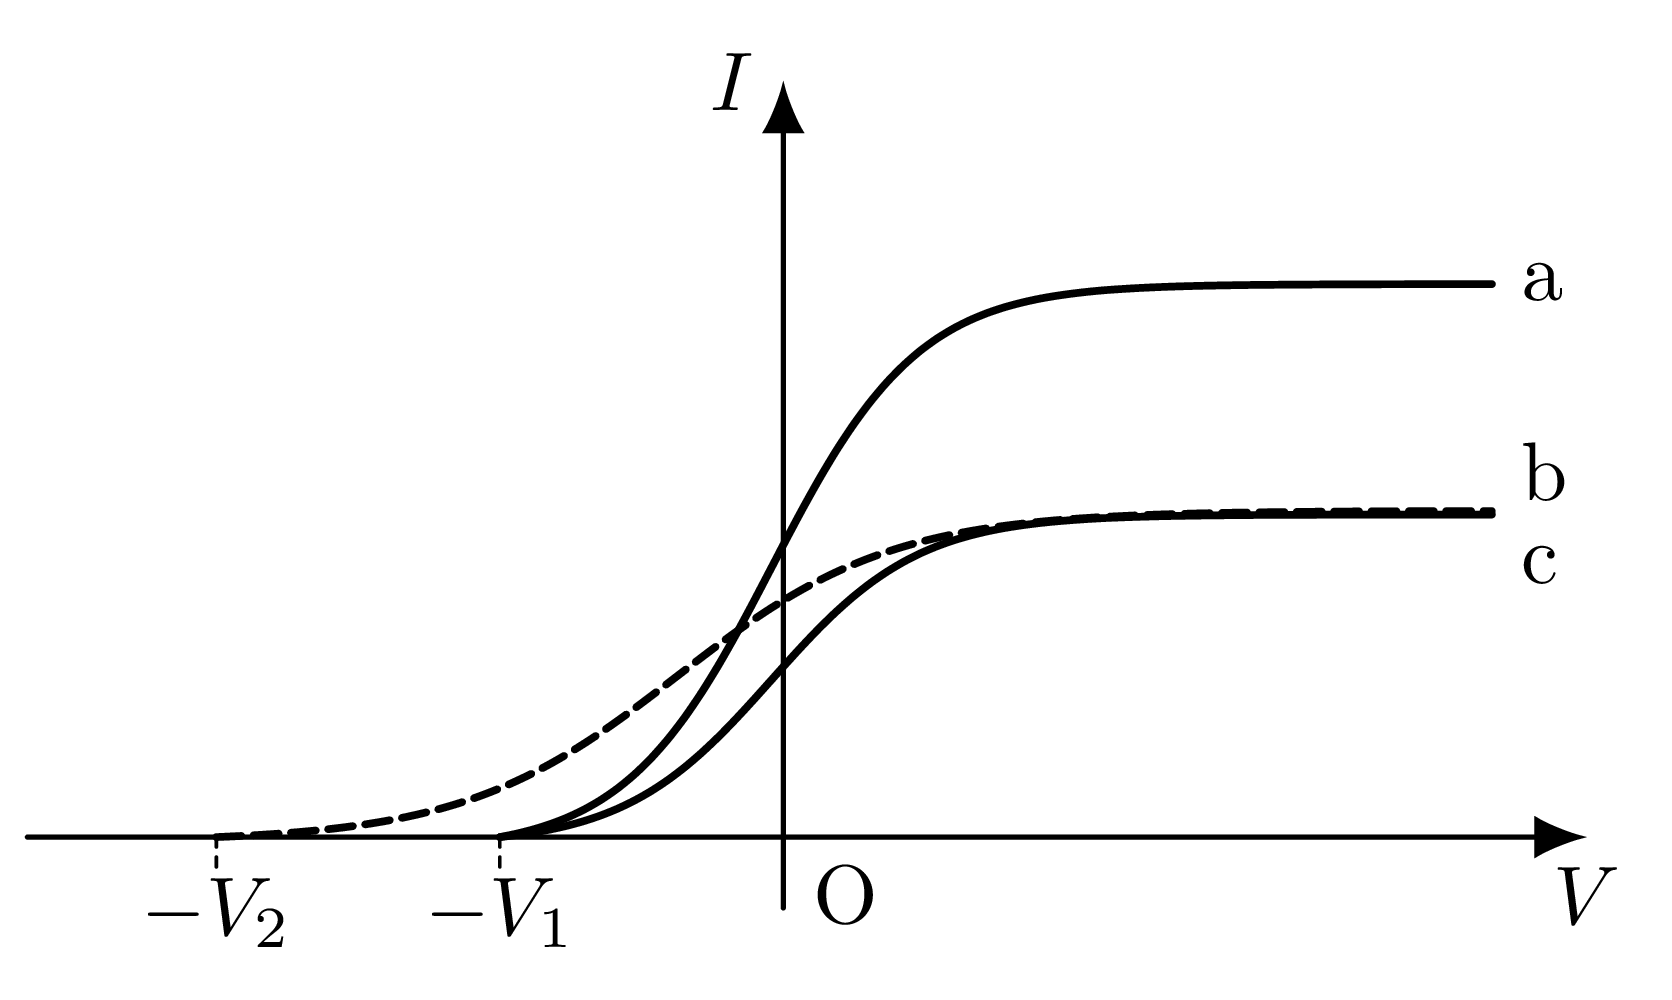
\includegraphics[keepaspectratio,width=52mm]{fig/n33_ex3_graph.png}
\end{zuright}
\end{reidai}

\begin{sisinE}
(1) 限界波長$500\U{nm}$から仕事関数が分かる．
(2) 電流が$0$になる電圧（阻止電圧）は$K_{\max}$，すなわち光の振動数を反映し，飽和電流は光子の数を反映する．
\end{sisinE}

\Key{$h\nu=K_{\max}+W$\quad 阻止電圧\ $\to$\ $K_{\max}$（振動数）を反映，飽和電流\ $\to$\ 光子の数を反映}

\begin{kaitou}
\begin{komon}
\ko{1} 限界波長を$\lambda_0=500\U{nm}$とすると$W=\dfrac{hc}{\lambda_0}$．波長$\lambda=400\U{nm}$の光では
       \[\frac{1}{2}mv_{\max}^2=\frac{hc}{\lambda}-\frac{hc}{\lambda_0}=hc\Bigl(\frac{1}{400\times 10^{-9}}-\frac{1}{500\times 10^{-9}}\Bigr)\fallingdotseq 9.95\times 10^{-20}\U{J}\]
       \[v_{\max}=\sqrt{\frac{2\times 9.95\times 10^{-20}}{9.11\times 10^{-31}}}\fallingdotseq 4.67\times 10^5\U{m/s}\Ans\]
\ko{2} 負の電圧で電流が減少して$0$になっているので，負の電圧は集電子板が受光板より低電位の場合である．よって横軸は\quad \MARU{2}\Ans\par
       阻止電圧が大きいほど$K_{\max}$が大きく，振動数が大きい．飽和電流が大きいほど光電子の数，すなわち光子の数が多い．よって
       \[\text{振動数：}\ \nu_{\mathrm{a}}=\nu_{\mathrm{b}}<\nu_{\mathrm{c}},\qquad\text{光子数：}\ N_{\mathrm{a}}>N_{\mathrm{b}}=N_{\mathrm{c}}\Ans\]
\end{komon}
\end{kaitou}
\end{reidaiunit}

\subsection{コンプトン効果}

コンプトン効果とは，光子が運動量を持つため，波長の短い電磁波（X線など）が電子と衝突する際に起こる現象である．
通常の可視光がちりなどに衝突して散乱される場合，光の進行方向のみが変化するだけでその波長は変化しない．
しかし，X線などの短波長の電磁波が電子に衝突して散乱される場合，光の進行方向が変わるとともにその波長も同時に変化し，しかも電子が動き出してしまう．
この現象は，{\gtfamily 光子が運動量$p=\dfrac{h\nu}{c}=\dfrac{h}{\lambda}$を持つ}と考えるとうまく説明できる．光子と電子の衝突を，力学の2物体の衝突と同じように扱えばよい．

%%%%%%%%%%  例題4（原本の【例題4】）  %%%%%%%%%%%%%%%%%%%%
\bsNeed{70mm}
\begin{reidaiunit}
\begin{reidai}{コンプトン効果}
\begin{zuright}{56mm}
\hspace{1zw}X線などの短波長の電磁波を電子に当てると，電子ははね飛ばされ，散乱されたX線の波長が変化する．この現象をコンプトン効果と呼ぶ．今，波長$\lambda\U{m}$の光子（X線）が，静止している電子（質量$m\U{kg}$）に衝突し，その結果，光子はその入射方向に対して角$\theta$の方向に散乱され，その波長が$\lambda^\prime\U{m}$に変化した．また，電子は光子の入射方向に対して角$\varphi$の方向に速さ$v\U{m/s}$で飛んでいった．プランク定数を$h\U{J\cdot s}$，光速を$c\U{m/s}$として，以下の設問に答えよ．
\zusep
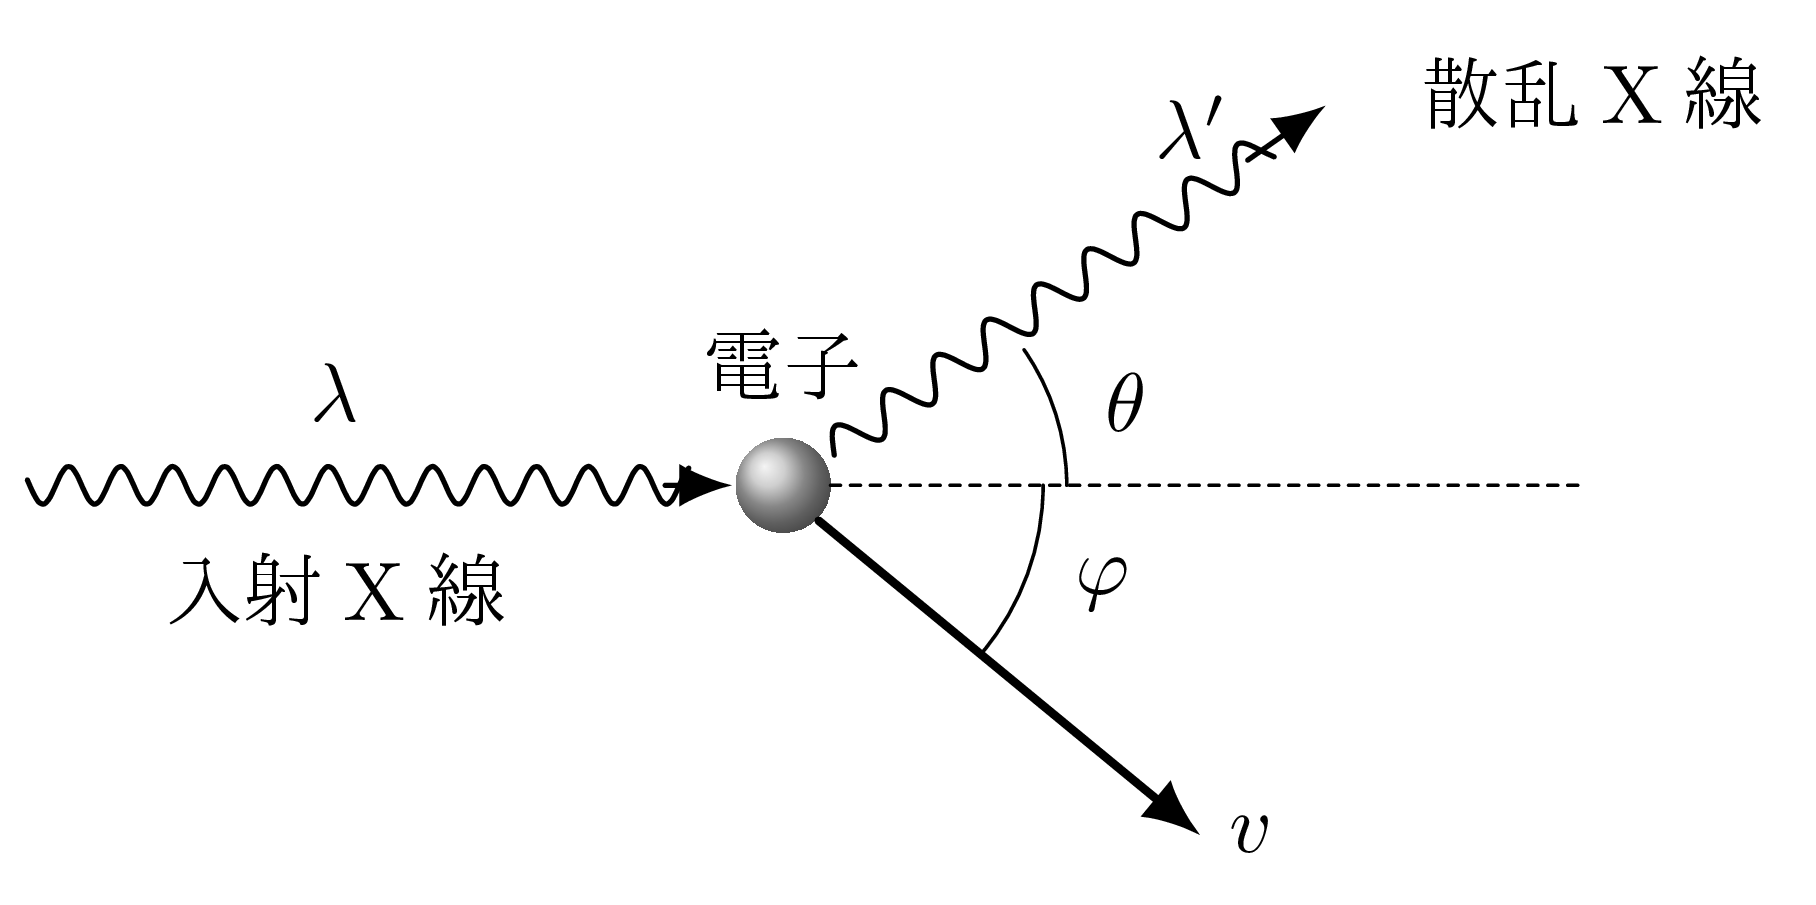
\includegraphics[keepaspectratio,width=54mm]{fig/n33_ex4_zu.png}
\end{zuright}
\begin{komon}
\ko{1} この衝突の前後のエネルギー保存則を式で示せ．
\ko{2} この衝突の前後の，入射方向およびそれに垂直な方向の運動量保存則を式で示せ．
\ko{3} 光子の波長の変化$\Delta\lambda=\lambda^\prime-\lambda$を，$h$，$m$，$c$，$\theta$を用いて表せ．ただし，$\lambda^\prime\fallingdotseq\lambda$のときに成り立つ近似式$\dfrac{\lambda}{\lambda^\prime}+\dfrac{\lambda^\prime}{\lambda}\fallingdotseq 2$を用いてよい．
\end{komon}
\end{reidai}

\begin{sisinE}
光子のエネルギー$\dfrac{hc}{\lambda}$と運動量$\dfrac{h}{\lambda}$を使って，2物体の衝突と同じように保存則を立てる．(3)は2つの式を満たすように変形すればよい．まず運動量保存則の2式から$\varphi$を消し（もしくは運動量ベクトルの図で余弦定理を用い），続いて$(mv)^2$を消去するように変形する．
\end{sisinE}

\Key{コンプトン効果\ $\Rightarrow$\ エネルギー保存則と運動量保存則とを組み合わせる}

\begin{kaitou}
\begin{komon}
\ko{1} \[\frac{hc}{\lambda}=\frac{hc}{\lambda^\prime}+\frac{1}{2}mv^2\Ans\]
\ko{2} \[\text{入射方向：}\ \frac{h}{\lambda}=\frac{h}{\lambda^\prime}\cos\theta+mv\cos\varphi,\qquad\text{垂直な方向：}\ 0=\frac{h}{\lambda^\prime}\sin\theta-mv\sin\varphi\Ans\]
\ko{3} (2)の2式から$\varphi$を消去すると（$\cos^2\varphi+\sin^2\varphi=1$）
       \[(mv)^2=\Bigl(\frac{h}{\lambda}\Bigr)^2+\Bigl(\frac{h}{\lambda^\prime}\Bigr)^2-\frac{2h^2}{\lambda\lambda^\prime}\cos\theta\]
       (1)より$(mv)^2=2mhc\Bigl(\dfrac{1}{\lambda}-\dfrac{1}{\lambda^\prime}\Bigr)$なので，両者を等しいとおいて両辺に$\dfrac{\lambda\lambda^\prime}{h}$をかけると
       \[h\Bigl(\frac{\lambda^\prime}{\lambda}+\frac{\lambda}{\lambda^\prime}-2\cos\theta\Bigr)=2mc(\lambda^\prime-\lambda)\]
       近似式を用いて
       \[\Delta\lambda=\lambda^\prime-\lambda=\frac{h}{mc}(1-\cos\theta)\Ans\]
\end{komon}
\end{kaitou}
\end{reidaiunit}

% 加筆：光の二重性（練習［1］(7)，［3］）．
光電効果・コンプトン効果は光の{\gtfamily 粒子性}を示す現象であり，一方で干渉・回折（第2章 波動）は光の{\gtfamily 波動性}を示す現象である．光は，粒子としての性質と波としての性質を併せ持っている（{\gtfamily 光の二重性}）．

\bsNeed{26mm}
\begin{matome}{光の二重性}
 \hspace{3mm} 粒子性を示す現象：\AnaB{光電効果}，\AnaB{コンプトン効果}\qquad 波動性を示す現象：\AnaB{干渉}，\AnaB{回折}
\end{matome}

\subsection{物質波}

振動数$\nu$，波長$\lambda$の光はエネルギー$E=h\nu$，運動量$p=\dfrac{h}{\lambda}$の，光子と呼ばれる粒子の性質を持つと同時に，光波と呼ばれる波の性質を併せ持つ．
これと同様に，電子のような質量の小さい粒子もまた，それに対応する波としての性質を併せ持っていることをド・ブロイは発見した．
エネルギー$E$，運動量$p$の物質に伴う波（{\gtfamily 物質波}）の振動数$\nu$および波長$\lambda$は
\[\nu=\frac{E}{h},\qquad\lambda=\frac{h}{p}\]
で与えられる．これを{\gtfamily ド・ブロイの関係}といい，$\lambda$を{\gtfamily ド・ブロイ波長}という．
特に，粒子の質量が$m$，速さが$v$であるときは，$p=mv$であるから
\[\lambda=\frac{h}{mv}\]
である．なお，$v$は波の伝わる速さではないので，$v=\nu\lambda$の関係式は成立しない点に注意すること．
電子線を結晶に当てると，X線と同じように回折・干渉が起こることが確かめられている（第34回のブラッグ反射）．

\bsNeed{20mm}
\begin{matome}{ド・ブロイ波長}
 \hspace{3mm} 質量$m\U{kg}$，速さ$v\U{m/s}$の粒子は，波長\AnaB{$\lambda=\dfrac{h}{mv}$}$\U{m}$の物質波を伴う．
\end{matome}

%%%%%%%%%%  例題5（原本の【例題5】）  %%%%%%%%%%%%%%%%%%%%
\bsNeed{40mm}
\begin{reidaiunit}
\begin{reidai}{物質波}
\hspace{1zw}静止していた電子を電圧$V\U{V}$で加速したときの電子線の波長を求めよ．ただし，電気素量を$e\U{C}$，電子の質量を$m\U{kg}$，プランク定数を$h\U{J\cdot s}$とする．
\end{reidai}

\begin{sisinE}
加速された電子の運動量を，エネルギー保存則から求めればよい．
\end{sisinE}

\Key{ド・ブロイ波長\ $\lambda=\dfrac{h}{p}=\dfrac{h}{mv}$}

\begin{kaitou}
電圧$V$で加速された電子の運動エネルギーは$\dfrac{1}{2}mv^2=eV$なので，運動量は$mv=\sqrt{2meV}$．よって
\[\lambda=\frac{h}{mv}=\frac{h}{\sqrt{2meV}}\U{m}\Ans\]
\end{kaitou}
\end{reidaiunit}

\subsection{トムソンの原子模型とラザフォードの原子模型}

物質は原子という，それ以上分割できない粒子から構成されているという概念は古くから存在したが，1897年にトムソンによって電子の比電荷が測定され，同年にゼーマンによって電子が原子内に含まれていることが確認されると，原子内に電子がどのように存在するかに興味が持たれた．

電子の質量は原子に比べて非常に小さく，また原子全体は電気的に中性であることから，原子から電子を取り除いた残りの部分は，原子の大部分の質量を持ち，かつ電子の負電荷を打ち消す正電荷を持ったものだと考えられる．
また，原子はある特定の波長・振動数の電磁波を吸収したり放出したりすることが当時知られていた．

\begin{zuright}{56mm}
\hspace{1zw}そこでトムソンは，正電荷が球状の原子いっぱいに雲のように一様に分布し，電子がこの中に埋め込まれて安定な状態でつり合って静止しているモデル（ブドウパンモデルとも呼ばれる）を考えた．
この場合，外部からの何らかの作用によって電子が安定位置からずれると，つり合いの位置を中心として振動し，その振動数と一致した電磁波を吸収・放出すると考えられる．
\zusep

\includegraphics[keepaspectratio,width=54mm]{text2_p102_fig1.png}
\end{zuright}

\begin{zuright}{52mm}
\hspace{1zw}ラザフォードの弟子であるガイガーとマースデンは，放射性元素ラジウムから放出される$\alpha$粒子（ヘリウムの原子核$\mathrm{{}^4_2He^{2+}}$）を厚さ約$0.5\U{\mu m}$の金箔に垂直に当て，その後の$\alpha$粒子の進行方向について調べた．
すると，大半の$\alpha$粒子はほとんど直進し，$10^5$個に1個程度の割合でごく一部の$\alpha$粒子が非常に大きく曲げられることが分かった．

\hspace{1zw}トムソンのモデルでは，原子の内部で正電荷がほぼ一様に分布していることから，$\alpha$粒子は大きな反発力を受けず，曲がるとしても曲がり方はわずかになるはずである．
進行方向に対して$90^\circ$以上方向を変えるような大きな散乱をするためには，$\alpha$粒子が大きな反発力を受ける必要がある．

\hspace{1zw}そこで，図にあるようなラザフォードのモデルを想定すると，大半の$\alpha$粒子は直進するが，ごくわずかの$\alpha$粒子が，極めて狭い部分に集中した正電荷のすぐそばを通り，大きな斥力を受けて進路を大きく変えたと考えられ，実験結果をうまく説明することができる．
\zusep

\includegraphics[keepaspectratio,width=50mm]{text2_p102_fig2.png}
\end{zuright}

\bsNeed{30mm}
\begin{matome}{ラザフォードの結論}
 \MARU{1}\ 原子の中心に，原子のほぼ全質量を持つ\AnaB{原子核}が存在する．\\
 \MARU{2}\ 原子番号$Z$の原子核は$+Ze$の正電荷を持つ．原子核の半径は電子の円運動半径の約$\dfrac{1}{10000}$である．\\
 \MARU{3}\ 原子核の周囲を$Z$個の電子が回っており，原子核の正電荷を中和して電気的に中性になっている．
\end{matome}

ところが，一見正しそうに見えるこのラザフォードのモデルにも次のような難点があった．
原子は特定の波長の電磁波を吸収・放射することが知られている．例えば水素原子の気体は下図のように，紫外線領域，可視光領域，赤外線領域にそれぞれ群をなして，ある特定の波長の電磁波のみを放射する．紫外部に現れる一群を{\gtfamily ライマン系列}，可視部に現れる一群を{\gtfamily バルマー系列}，赤外部に現れる一群を{\gtfamily パッシェン系列}という．
\begin{center}

\includegraphics[keepaspectratio,width=120mm]{text2_p103_fig1.png}
\end{center}

\begin{zuright}{36mm}
\hspace{1zw}ラザフォードのモデルを水素原子に適用してみよう．
水素原子は$+e$の電荷を持つ原子核のまわりを$-e$の電荷を持つ電子がクーロン力を受けて等速円運動していると考えられる．電子の速さを$v$，質量を$m$，軌道半径を$r$とすると，運動方程式は
\[m\frac{v^2}{r}=k\frac{e^2}{r^2}\]
であり，電子の持つエネルギーは運動エネルギーとクーロン力による位置エネルギーの和であるから
\[E=\frac{1}{2}mv^2-k\frac{e^2}{r}=-\frac{ke^2}{2r}\quad\cdots\text{(☆)}\]
となる．
\zusep

\includegraphics[keepaspectratio,width=34mm]{text2_p103_fig2.png}
\end{zuright}

\begin{zuright}{48mm}
\hspace{1zw}電磁気学によると，電荷を持ったものが円運動すると，その回転数に等しい振動数の電磁波を放出して，エネルギーを失うことが知られている．$E$が減少すると，(☆)式から$r$が減少し，電子はやがて原子核に落ち込んでしまう．
すなわち，{\gtfamily ラザフォードモデルでは原子の大きさが定まらない}という難点がある．
また，発せられる電磁波の振動数は$\nu=\dfrac{v}{2\pi r}\propto\dfrac{1}{\sqrt{r^3}}$となるため，$r$の減少とともに$\nu$は連続的に大きくなる．しかし実際には，原子はある特定の振動数の電磁波しか出さない．
すなわち，{\gtfamily ラザフォードモデルでは原子の発する電磁波が連続的に変化してしまう}という難点がある．
\zusep

\includegraphics[keepaspectratio,width=46mm]{text2_p104_fig1.png}
\end{zuright}

このような問題が生じてしまうのは，通常の電磁気学を原子内の電子という非常に微細な粒子に対して適用してしまったからであり，次に述べるボーアの理論によりこれらの難点はすべて解決される．

\subsection{ボーアの水素原子モデル}

\begin{zuright}{56mm}
\hspace{1zw}ラザフォードモデルの難点を，ボーアは次の3つの仮定を持ち出すことで見事に解決することに成功した．
\begin{description}
\item[\MARU{1}] {\gtfamily 電子が原子内で持つエネルギーは連続的にすべての値をとりうるのではなく，いくつかの特定のエネルギー値しか持たない．また，そのエネルギーを持った状態にある限り，電磁波の放射は起こらない．}この状態を{\gtfamily 定常状態}といい，そのエネルギー値を{\gtfamily エネルギー準位}という．
\item[\MARU{2}] {\gtfamily 電子の軌道円上に電子波の定常波が実現するときに定常状態となる．}すなわち，電子のド・ブロイ波長を$\lambda$とするとき
\[2\pi r=n\lambda\quad(n=1,2,3,\cdots)\]
が成立する半径$r$のところにしか電子は安定に存在できない．これを{\gtfamily 量子条件}，$n$を{\gtfamily 量子数}という．$n$の値に応じて$r$，$E$が決まるので，これらを$r_n$，$E_n$と表す．
\end{description}
\zusep

\includegraphics[keepaspectratio,width=54mm]{text2_p104_fig2.png}
\end{zuright}

\begin{zuright}{56mm}
\begin{description}
\item[\MARU{3}] {\gtfamily 電子がエネルギー準位$E_n$の定常状態から$E_{n^\prime}$の定常状態に移るとき，そのエネルギー差$|E_n-E_{n^\prime}|$に等しいエネルギーの光子のみを吸収または放出する．}すなわち
\[h\nu=|E_n-E_{n^\prime}|\]
を満たす振動数$\nu$の光子を吸収または放出する．これを{\gtfamily 振動数条件}という．このため，吸収・放出される光の振動数は限定される．
\end{description}
% 原本の打ち込み（physics_ch44.tex）は「光子を吸収して電子がより低い準位に移動することを放射」と脱落していた．OCR により直した．
\hspace{1zw}右図のように，光子を吸収して電子がよりエネルギーの高い準位に移ることを{\gtfamily 励起}，逆に光子を放出して電子がよりエネルギーの低い準位に移ることを{\gtfamily 放射}（放出）という．また，電子がエネルギー準位間を移ることを{\gtfamily 遷移}という．
\zusep

\includegraphics[keepaspectratio,width=54mm]{text2_p105_fig1.png}
\end{zuright}

この3つの仮定から得られる水素原子の電子の軌道半径やエネルギー準位を用いると，水素原子の放出する電磁波を見事に説明することができる（例題6）．

%%%%%%%%%%  例題6（原本の【例題6】）  %%%%%%%%%%%%%%%%%%%%
\bsNeed{70mm}
\begin{reidaiunit}
\begin{reidai}{水素原子モデル}
\hspace{1zw}最も簡単な水素原子のモデルとして有名なものにボーア模型がある．このボーア模型は，電荷$+e\U{C}$の水素原子核のまわりを電荷$-e\U{C}$，質量$m\U{kg}$の電子が等速円運動をしているものとして与えられる．クーロンの法則の比例定数を$k\U{N\cdot m^2/C^2}$，プランク定数を$h\U{J\cdot s}$として以下の問いに答えよ．
\begin{komon}
\ko{1} 電子の円運動の軌道半径を$r\U{m}$，等速円運動の速さを$v\U{m/s}$として，電子の運動方程式を示せ．
\ko{2} 電子の持つ力学的エネルギーを$m$，$v$，$k$，$e$，$r$で表し，(1)を用いて$e$，$r$，$k$で表せ．ただし，クーロン力による位置エネルギーは無限遠方を基準点にとるものとする．
\ko{3} 等速円運動する電子の物質波としての波長$\lambda\U{m}$を，$h$，$m$，$v$を用いて表せ．
\ko{4} 電子の軌道としては，$r$，$\lambda$の間にある関係が成立するものだけが実現可能である．これを量子条件というが，これを$r$，$\lambda$および自然数$n$（量子数）を用いて表せ．
\ko{5} (1)〜(4)を用いて，量子数$n$の電子の軌道半径$r_n\U{m}$を$n$，$h$，$k$，$m$，$e$を用いて表せ．
\ko{6} 電子のエネルギー準位$E_n\U{J}$を$n$，$h$，$k$，$m$，$e$を用いて表せ．
\end{komon}
\end{reidai}

\begin{sisinE}
水素原子の半径・エネルギーの計算では，\MARU{1}運動方程式，\MARU{2}量子条件，\MARU{3}力学的エネルギーの式，の3つの式を組み合わせて計算する．
\end{sisinE}

\Key{水素原子\ $\Rightarrow$\ \MARU{1}運動方程式$m\dfrac{v^2}{r}=k\dfrac{e^2}{r^2}$\quad \MARU{2}量子条件$2\pi r=n\dfrac{h}{mv}$\quad \MARU{3}$E=\dfrac{1}{2}mv^2-k\dfrac{e^2}{r}$}

\begin{kaitou}
\begin{komon}
\ko{1} \[m\frac{v^2}{r}=k\frac{e^2}{r^2}\Ans\]
\ko{2} \[E=\frac{1}{2}mv^2-k\frac{e^2}{r}=\frac{1}{2}\cdot\frac{ke^2}{r}-\frac{ke^2}{r}=-\frac{ke^2}{2r}\U{J}\Ans\]
\ko{3} \[\lambda=\frac{h}{mv}\U{m}\Ans\]
\ko{4} \[2\pi r=n\lambda\Ans\]
\ko{5} (3)(4)より$mv=\dfrac{nh}{2\pi r}$．(1)より$mv^2=\dfrac{ke^2}{r}$なので，$(mv)^2=m\cdot mv^2$から$\dfrac{n^2h^2}{4\pi^2r^2}=\dfrac{mke^2}{r}$．よって
       \[r_n=\frac{h^2}{4\pi^2kme^2}\cdot n^2\U{m}\Ans\]
\ko{6} (2)に(5)を代入して
       \[E_n=-\frac{ke^2}{2r_n}=-\frac{2\pi^2k^2me^4}{h^2}\cdot\frac{1}{n^2}\U{J}\Ans\]
\end{komon}
\end{kaitou}
\end{reidaiunit}

ここで，$n$は自然数であるから$r_n$，$E_n$は飛び飛びの値しかとることができず，また
\[r_1<r_2<r_3<\cdots,\qquad E_1<E_2<E_3<\cdots\]
なる関係になっている．一般にエネルギーは低いほど安定であるから，$n=1$の軌道に電子がいるとき水素原子は最も安定である．これを{\gtfamily 基底状態}という．それに対して，$n\geqq 2$の軌道に電子がいるときのことを{\gtfamily 励起状態}という．

\begin{zuright}{50mm}
\hspace{1zw}基底状態における水素の原子半径$r_1$を{\gtfamily ボーア半径}$a_0$といい，これを計算すると
\[a_0=\frac{h^2}{4\pi^2kme^2}\fallingdotseq 5.3\times 10^{-11}\U{m}\]
となり，水素原子の大きさは$0.1\U{nm}$程度であると分かる．また，このときのエネルギー$E_1$は
\[E_1=-\frac{2\pi^2k^2me^4}{h^2}\fallingdotseq -13.6\U{eV}\]
である．よって
\[r_n=n^2a_0,\qquad E_n=-\frac{13.6}{n^2}\U{eV}\]
と書くことができる．そのため，水素原子のエネルギー準位は上に行くほど間隔が狭まっていく．
$n\to\infty$は電子がはるか遠方へと去った場合，すなわちイオン化した場合に対応するので，$E_\infty-E_1\fallingdotseq 13.6\U{eV}$は水素原子の{\gtfamily イオン化エネルギー}である．
\zusep

\includegraphics[keepaspectratio,width=48mm]{text2_p106_fig1.png}
\end{zuright}

\bsNeed{22mm}
\begin{matome}{水素原子のエネルギー準位}
 \hspace{3mm} \AnaB{$E_n=-\dfrac{13.6}{n^2}$}$\U{eV}$\qquad イオン化エネルギー$E_\infty-E_1\fallingdotseq 13.6\U{eV}$
\end{matome}

% 加筆：電子の衝突による励起（練習［9］フランク・ヘルツの実験の前提）．
原子は光子を吸収するだけでなく，{\gtfamily 高速の電子などが衝突することによっても励起される}．電子の運動エネルギーが励起に必要なエネルギー（基底状態と第1励起状態のエネルギー差）より小さいと，原子は励起されず，電子は運動エネルギーを失わずにはね返される（{\gtfamily 弾性衝突}）．運動エネルギーがそれ以上になると，衝突で原子が励起され，電子はそのぶんの運動エネルギーを失う（{\gtfamily 非弾性衝突}）．
このことを確かめたのがフランクとヘルツの実験で（練習［9］），原子のエネルギー準位が飛び飛びであることの直接の証拠となった．

\subsection{水素原子の発光スペクトル}

ボーアの水素原子模型から導かれるエネルギー準位の式は，水素原子の発光スペクトルの系列を説明する．
量子数$n^\prime$の軌道から$n$の軌道（ただし$n^\prime>n$）へ電子が遷移する場合について考えよう．
$E_{n^\prime}>E_n$であり，電子が失った分に相当するエネルギーが光子として放出されるから
\[h\nu=\frac{hc}{\lambda}=E_{n^\prime}-E_n\]
これに$E_n$の式を代入し，波長$\lambda$の逆数を計算すると
\[\frac{1}{\lambda}=\frac{2\pi^2k^2me^4}{ch^3}\Bigl(\frac{1}{n^2}-\frac{1}{n^{\prime 2}}\Bigr)\]
が得られる．
% 加筆：リュードベリの式（練習［7］の前提）．
実は，ボーアの理論以前から，水素原子のスペクトルの波長は実験的に
\AnaBD{\frac{1}{\lambda}=R\Bigl(\frac{1}{n^2}-\frac{1}{n^{\prime 2}}\Bigr)}
と表せることが知られていた（{\gtfamily リュードベリの式}）．$R\fallingdotseq 1.1\times 10^7\U{/m}$を{\gtfamily リュードベリ定数}という．ボーアの理論は，この$R$を$R=\dfrac{2\pi^2k^2me^4}{ch^3}$として導き出したのである．

\begin{zuright}{50mm}
\hspace{1zw}この式で$n=1,2,3$とおき，$n^\prime$に$n$より大きい整数を代入して波長を計算すると，それぞれライマン系列，バルマー系列，パッシェン系列の波長と一致する．
すなわち，{\gtfamily ライマン系列は$n=1$の軌道へ，バルマー系列は$n=2$の軌道へ，パッシェン系列は$n=3$の軌道へ電子が遷移するときに放出される光子}であるとまとめることができる．こうしてボーアは，ラザフォード模型の問題点を解決すると同時に，原子の放出する電磁波の波長を説明することに成功した．
\zusep

\includegraphics[keepaspectratio,width=48mm]{text2_p107_fig1.png}
\end{zuright}

\bsNeed{24mm}
\begin{matome}{水素原子のスペクトル}
 \hspace{3mm} $h\nu=E_{n^\prime}-E_n$\quad $\dfrac{1}{\lambda}=R\Bigl(\dfrac{1}{n^2}-\dfrac{1}{n^{\prime 2}}\Bigr)$\qquad 遷移先$n=1$：\AnaB{ライマン}，$n=2$：\AnaB{バルマー}，$n=3$：\AnaB{パッシェン}系列
\end{matome}

%%%%%%%%%%  例題7（原本の【例題7】）  %%%%%%%%%%%%%%%%%%%%
\bsNeed{70mm}
\begin{reidaiunit}
\begin{reidai}{水素原子のスペクトル}
\begin{zuright}{52mm}
\hspace{1zw}水素原子から出された光子を調べたところ，振動数が\MARU{1}\ $\nu_1=4.57\times 10^{14}\U{Hz}$，\MARU{2}\ $\nu_2=7.32\times 10^{14}\U{Hz}$の2つの光子が観察された．水素原子のエネルギー準位を図示した右図を利用して，以下の設問に答えよ．ただし，電気素量を$1.60\times 10^{-19}\U{C}$，プランク定数を$6.63\times 10^{-34}\U{J\cdot s}$とする．
\begin{komon}
\ko{1} \MARU{1}，\MARU{2}の電磁波はそれぞれどのエネルギー準位からどのエネルギー準位に遷移するときに放出されたものか．
\ko{2} \MARU{1}，\MARU{2}はそれぞれ何系列に属する光子か．
\end{komon}
\zusep
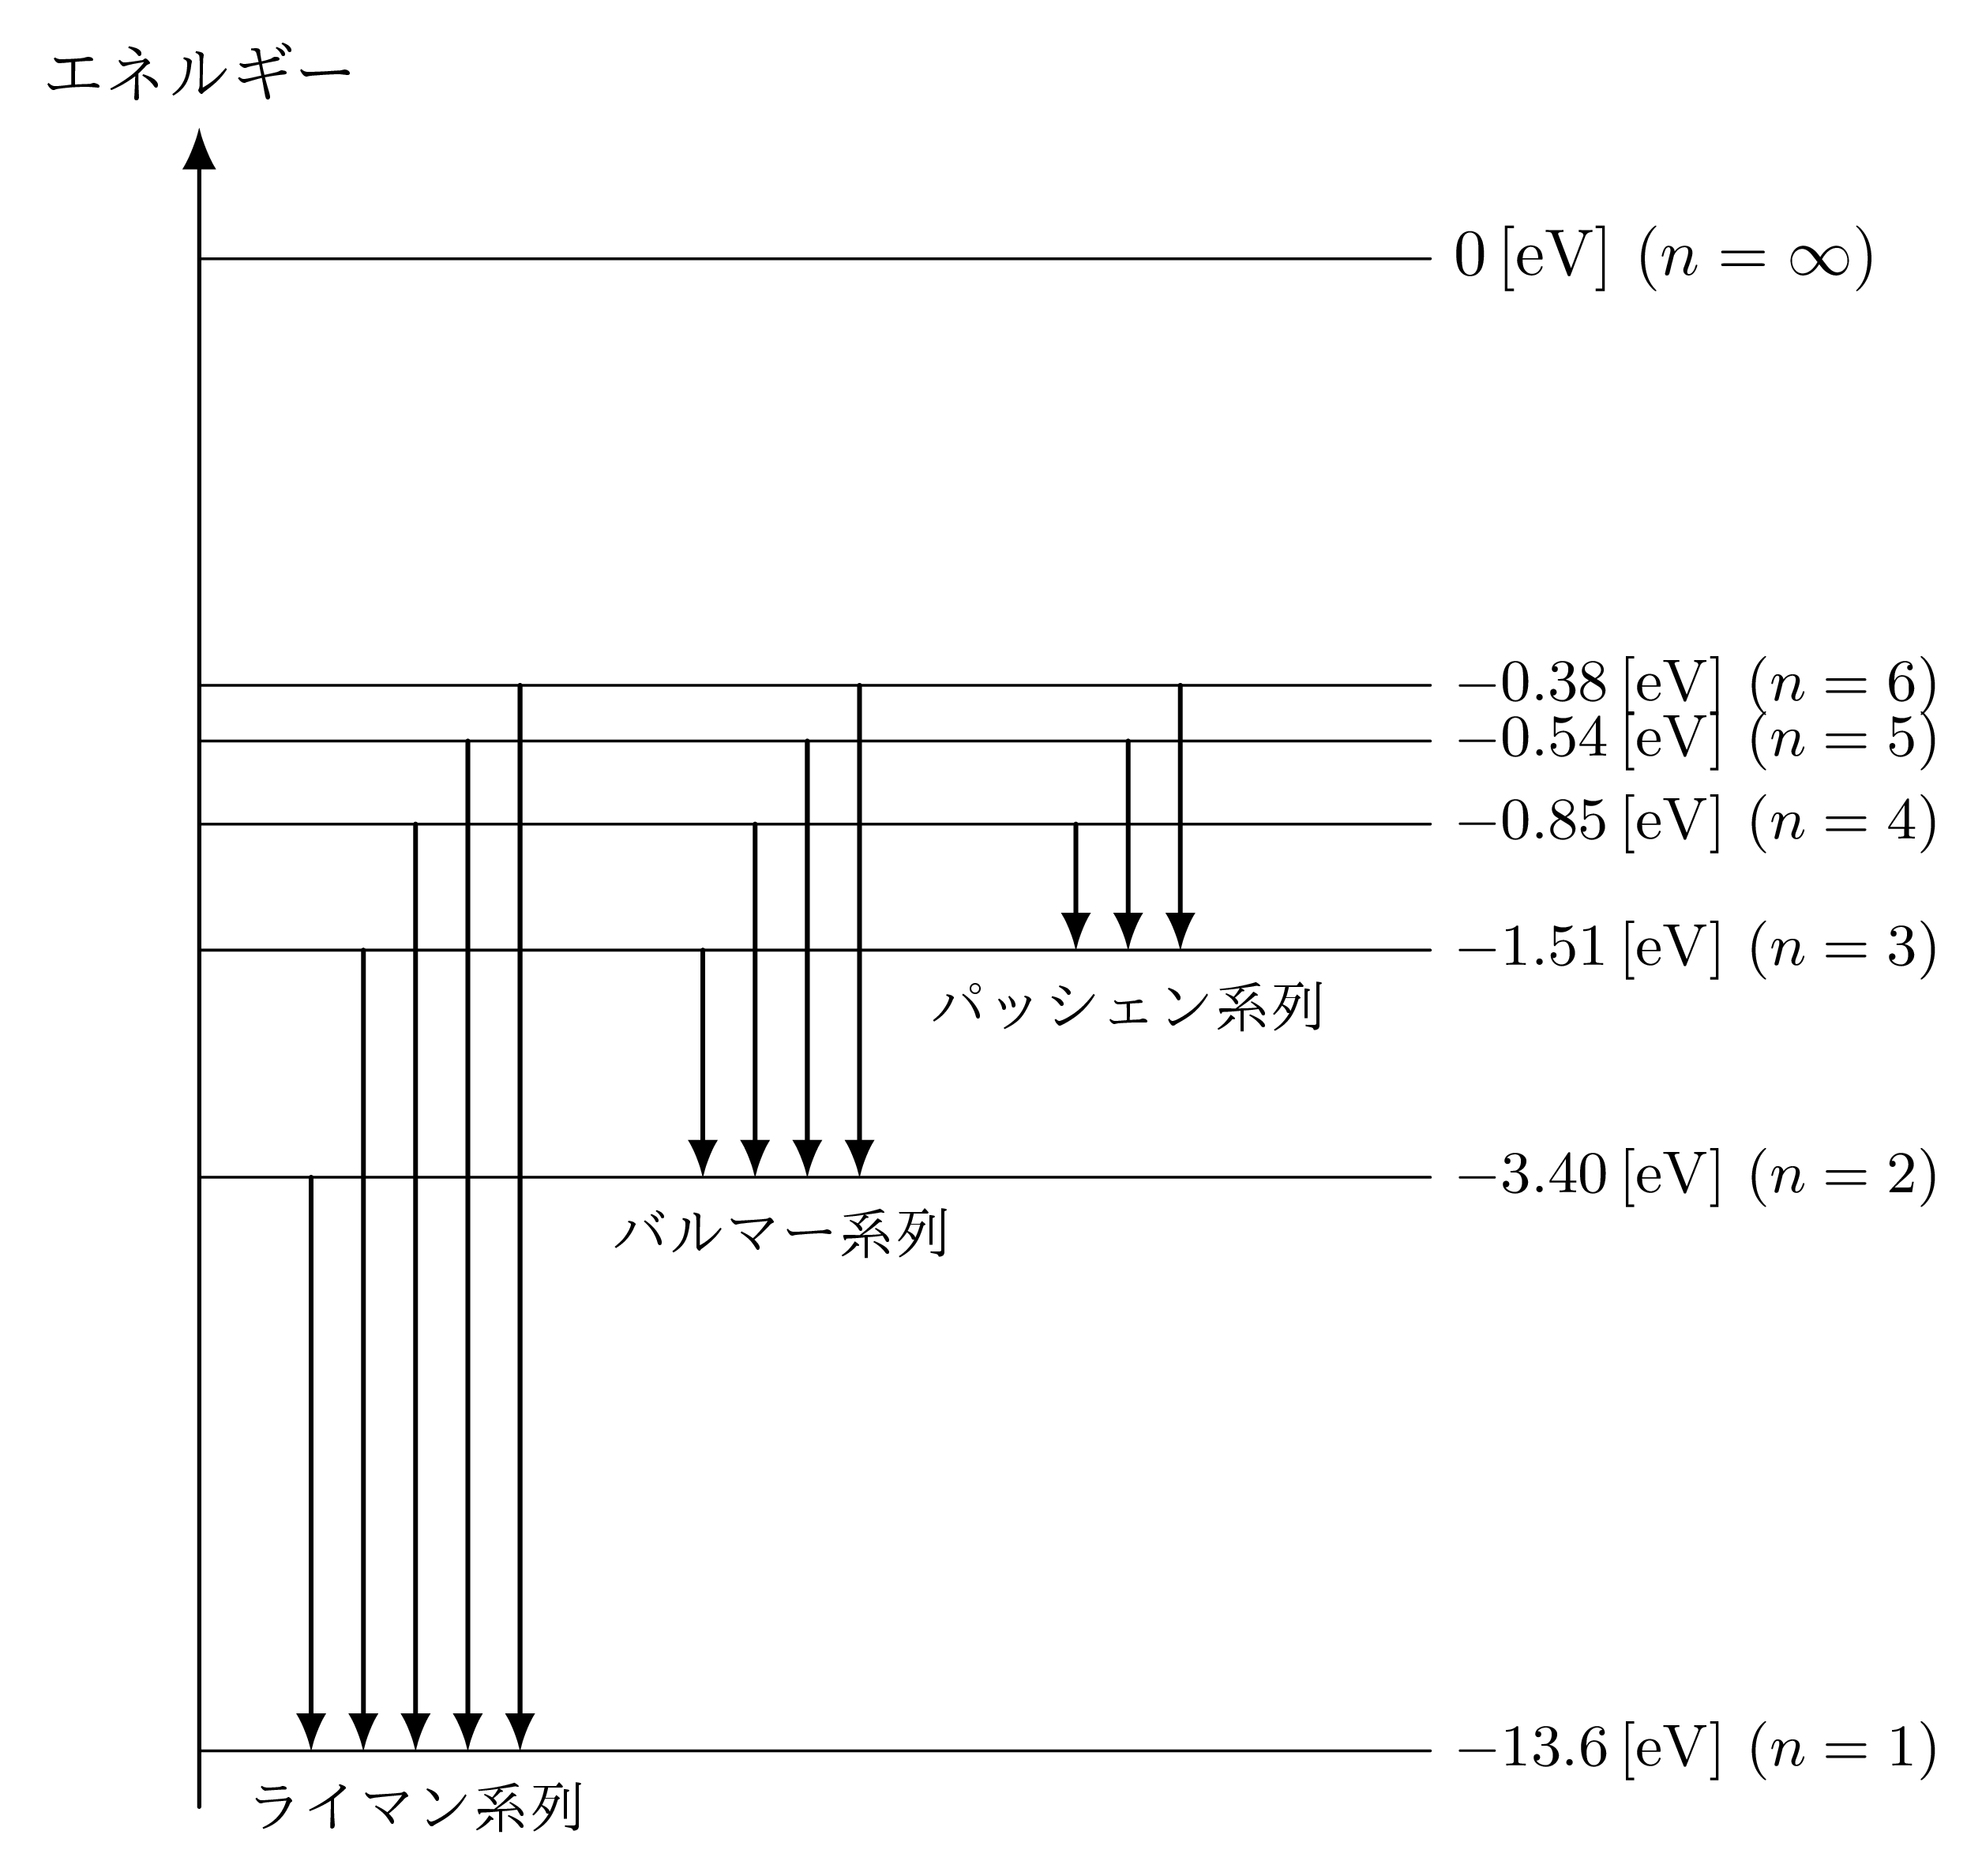
\includegraphics[keepaspectratio,width=50mm]{fig/n33_ex7_level.png}
\end{zuright}
\end{reidai}

\begin{sisinE}
まず光子のエネルギーを$\U{eV}$単位で計算し，それがどの2つの準位の間の差に等しいかを考えよ．
\end{sisinE}

\Key{振動数条件\ $h\nu=E_{n^\prime}-E_n$\quad 遷移先が$n=1$：ライマン，$n=2$：バルマー，$n=3$：パッシェン}

\begin{kaitou}
\begin{komon}
\ko{1} 光子のエネルギーを$\U{eV}$単位で表すと
       \[h\nu_1=\frac{6.63\times 10^{-34}\times 4.57\times 10^{14}}{1.60\times 10^{-19}}\fallingdotseq 1.89\U{eV},\qquad h\nu_2=\frac{6.63\times 10^{-34}\times 7.32\times 10^{14}}{1.60\times 10^{-19}}\fallingdotseq 3.03\U{eV}\]
       $-1.51-(-3.40)=1.89\U{eV}$，$-0.38-(-3.40)=3.02\U{eV}$より，\MARU{1}は{\gtfamily $n=3\to n=2$}，\MARU{2}は{\gtfamily $n=6\to n=2$}の遷移．\Ans
\ko{2} どちらも$n=2$の準位への遷移なので，\MARU{1}\MARU{2}とも{\gtfamily バルマー系列}．\Ans
\end{komon}
\end{kaitou}
\end{reidaiunit}




\newpage

%%%%%%%%%%%%%%%%%%%%  練習問題  %%%%%%%%%%%%%%%%%%%%
% 原子物理の練習番号は章の先頭から［1］〜
\setcounter{qno}{0}

\filbreak
\Rank{A問題}

\Mon{基本事項の確認}

\hspace{1zw}以下の設問に答えよ．電子の質量は$m_e=9.1\times 10^{-31}\U{kg}$，電気素量は$e=1.6\times 10^{-19}\U{C}$，プランク定数は$h=6.63\times 10^{-34}\U{J\cdot s}$，光速は$c=3.0\times 10^8\U{m/s}$である．
\begin{komon}
\ko{1} $0.10\U{m}$だけ離れた平行極板に$2.0\times 10^2\U{V}$の電圧をかけた．初速度$0\U{m/s}$でこの平行極板の負極から飛び出した電子が正極に達したときの電子の速さは何$\U{m/s}$か．
\ko{2} ミリカンの実験で，油滴に帯電している電荷に対して，次のような実験結果を得た．この実験結果から推定される電気素量$e$は何$\U{C}$か．\\
       \hspace*{2zw}油滴の電荷$q$（数値の単位は$10^{-19}\U{C}$）：$4.86$，$8.05$，$9.67$，$11.25$，$16.02$
\ko{3} 波長$6.0\times 10^{-7}\U{m}$の光の光子1個が持っているエネルギーは何$\U{J}$か．またこの光子の運動量は何$\U{kg\cdot m/s}$か．
\ko{4} 限界振動数が$\nu_0=3.3\times 10^{14}\U{Hz}$である金属の仕事関数$W$は何$\U{J}$か．
\ko{5} 光電効果が起こる限界の光の色が緑の金属に赤色の光を当てると，この金属から電子は飛び出すか．また紫色の光ではどうか．
\ko{6} 陰極物質の限界振動数が$\nu_0=3.3\times 10^{14}\U{Hz}$の光電管に振動数$\nu=5.0\times 10^{14}\U{Hz}$の単色光を照射した．このとき陰極から放出される光電子の速さの最大値は何$\U{m/s}$か．
\ko{7} 光の粒子性および波動性からよく説明される光学的現象をそれぞれ2つずつあげよ．
\ko{8} 速さ$1.0\times 10^7\U{m/s}$で運動している電子に伴う物質波の波長は何$\U{m}$か．
\ko{9} ラザフォードは，放射性物質から放射される$\alpha$線を金属に当てたときの散乱の様子から，どのようなことを結論したか．
\ko{10} 水素原子内の電子が$-0.85\U{eV}$のエネルギー準位から，$-3.40\U{eV}$のエネルギー準位に遷移するとき，放出される光子のエネルギーは何$\U{J}$か．またこの光子の振動数は何$\U{Hz}$か．
\end{komon}

\filbreak
\Rank{B問題}

\Mon[\Sitei]{ミリカンの実験}

\begin{zuright}{40mm}
\hspace{1zw}図のような上下2枚の水平な極板$\mathrm{PQ}$間で落下する質量$m\U{kg}$の油滴に注目しよう．油滴の運動に対する空気の抵抗は油滴の速さ$v\U{m/s}$に比例し，大きさが$kv\U{N}$で表されるものとする．空気の浮力は無視できるものとし，$\mathrm{PQ}$間は十分な距離がある．重力加速度の大きさを$g\U{m/s^2}$として，以下の設問に答えよ．
\zusep
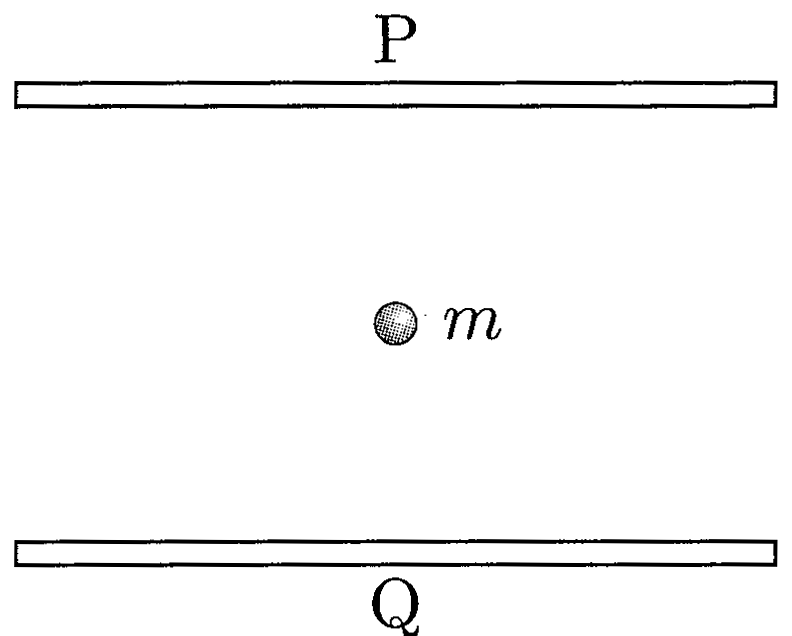
\includegraphics[keepaspectratio,width=36mm]{fig/n33_p2_zu.png}
\end{zuright}
\begin{komon}
\ko{1} まず，$\mathrm{PQ}$間に電圧がかかっていない場合について考える．この場合，油滴は重力により加速されて落下するが，十分に時間がたてば油滴は一定の速さ（終端速度）で下降するようになる．この終端速度の大きさ$v_0\U{m/s}$を，終状態において油滴にかかる力を元にして求めよ．
\ko{2} 油滴に適当な正電荷$q\U{C}$を与え，$\mathrm{PQ}$間に電圧をかけて極板間に一様な電場を上向きにかけた．電場を適当な大きさに調節すれば油滴を静止させることができる．油滴が静止することのできる電場の大きさ$E_0\U{N/C}$を求めよ．
\ko{3} 以上より，この油滴の電荷$q\U{C}$を，$v_0$および$E_0$を用いて表せ．
\end{komon}

\Mon[\Sitei]{光電効果}

\hspace{1zw}以下は光電効果について述べた文章である．\framebox[3zw]{\rule{0pt}{1.1zw}}内を適切な語句や数式で埋めよ．ただし，プランク定数を$h\U{J\cdot s}$，真空中での光の速さを$c\U{m/s}$とする．選択肢が書かれているものは正しいものを選んで答えよ．
\par
\hspace{1zw}金属表面に光を照射すると電子が飛び出すことがある．これを光電効果という．この現象は，光を，質量\BOX{1}\Sentaku{を持ち／は持たないが}，エネルギーを持つ粒子，すなわち\BOX{2}と考えることによって説明される．これに対して，光の\BOX{3}や\BOX{4}などの現象は，むしろ光を\BOX{5}と考えるとうまく説明ができる．
\par
\hspace{1zw}\BOX{2}のエネルギー$\varepsilon\U{J}$は，光の振動数を$\nu\U{Hz}$とすると，$\varepsilon=$\BOX{6}と表され，また運動量の大きさ$p\U{kg\cdot m/s}$は，$p=$\BOX{7}と表される．
\par
\hspace{1zw}光電効果によって金属表面から飛び出した電子を\BOX{8}という．光電効果において，1つの\BOX{2}のエネルギーが金属内の2つ以上の電子に配分されること\BOX{9}\Sentaku{はない／もある}．
\par
\hspace{1zw}\BOX{2}からエネルギーをもらった電子が，金属表面の外に飛び出してくるまでの間に失われるエネルギーのうち，\BOX{10}\Sentaku{最大／最小}のエネルギーを\BOX{11}という．これは金属の種類に\BOX{12}\Sentaku{よらず一定である／よって異なる}．
\par
\hspace{1zw}\BOX{11}が$W\U{J}$である金属に振動数$\nu\U{Hz}$の光を照射した際に出てくる電子のうち，最大運動エネルギーを持つ電子の運動エネルギー$K_{\max}\U{J}$は$K_{\max}=$\BOX{13}である．また，この金属に光を照射して光電効果を起こすために必要な光の振動数は\BOX{14}\BOX{15}\Sentaku{以上／以下}であり，波長で言えば\BOX{16}\BOX{17}\Sentaku{以上／以下}である．これらの値をそれぞれ\BOX{18}，\BOX{19}という．

\Mon[\Sitei]{光電管}

\begin{zuright}{50mm}
\hspace{1zw}図1は光電効果を調べる装置である．一定の強度，振動数$\nu\U{Hz}$の光を電極$\mathrm{C}$に当てながら制御電圧$V\U{V}$を変えて，回路に流れる電流$I\U{A}$を調べたところ，図2のようなグラフが得られた．これについて以下の設問に答えよ．ただし，電子の質量を$m\U{kg}$，電気素量を$e\U{C}$，プランク定数を$h\U{J\cdot s}$，光速を$c\U{m/s}$とする．
\zusep
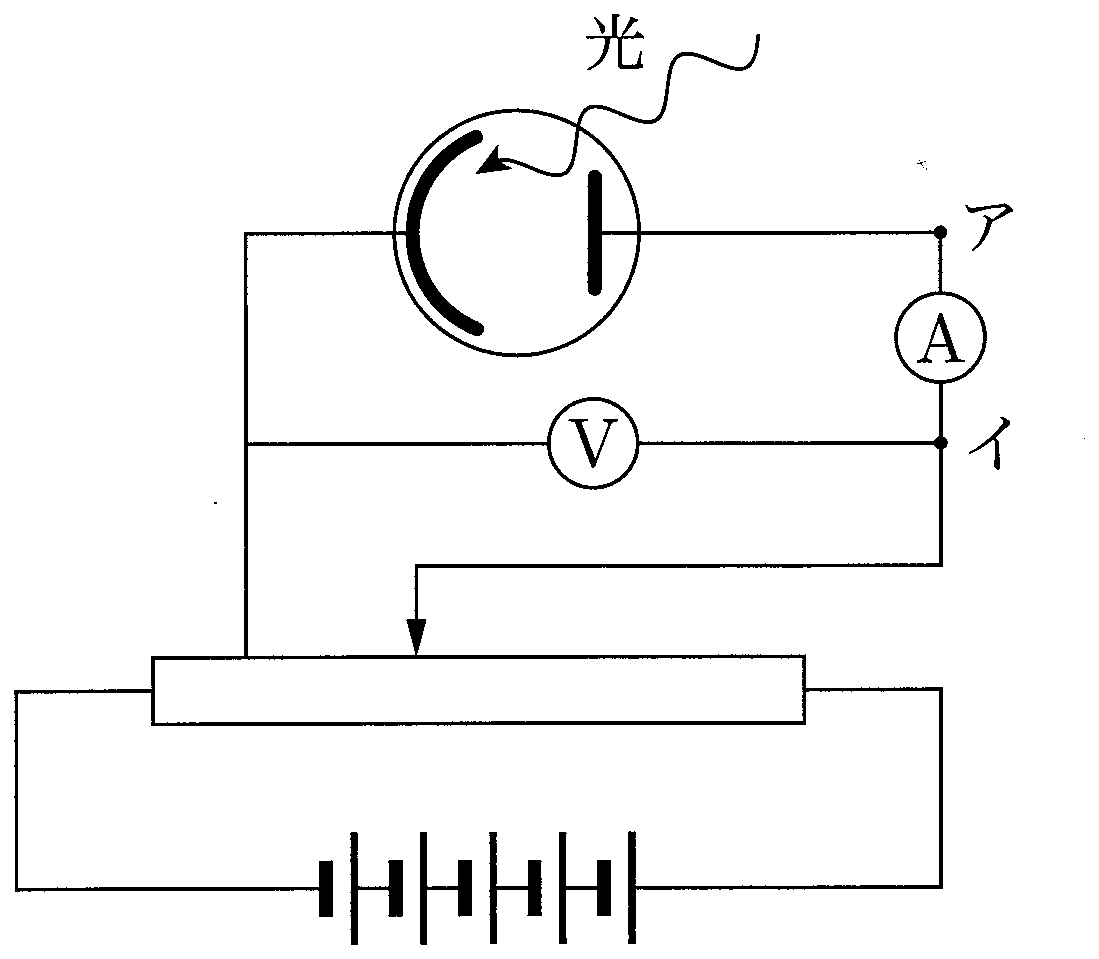
\includegraphics[keepaspectratio,width=46mm]{fig/n33_p4_zu1.png}\\{\small 図1}
\end{zuright}
\begin{komon}
\ko{1} 電流$I$の向きは図のア$\to$イ，イ$\to$アのどちらか．
\ko{2} 制御電圧$V$を十分大きくして電流$I$が飽和したとき，電流量が$I_0\U{A}$になった．このとき，陰極表面から単位時間あたりに出てくる電子の個数はいくらか．
\ko{3} 光がこの振動数のとき，阻止電圧が$-V_{\mathrm{S}}\U{V}$であった．電極$\mathrm{C}$から出てくる電子の速さのうち，最大の値はいくらか．
\end{komon}
\begin{zuright}{70mm}
\hspace{1zw}次に，光の振動数$\nu\U{Hz}$をいろいろに変えて図2の阻止電圧$-V_{\mathrm{S}}$を測定し，これをグラフ化したところ，図3の実線部分を得た．
\begin{komon}
\ko{4} グラフの傾きはいくらか．
\ko{5} グラフの直線を延ばした$V$軸との交点を$-V_0\U{V}$とおく．このとき，$eV_0$の値は何を表すか．
\ko{6} グラフの$\nu$軸切片は何を表すか．
\end{komon}
\zusep
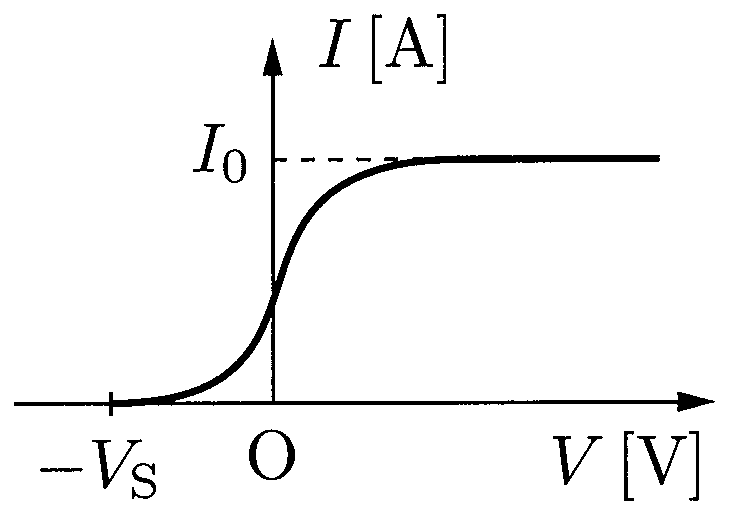
\includegraphics[keepaspectratio,width=36mm]{fig/n33_p4_zu2.png}\hspace{2mm}%
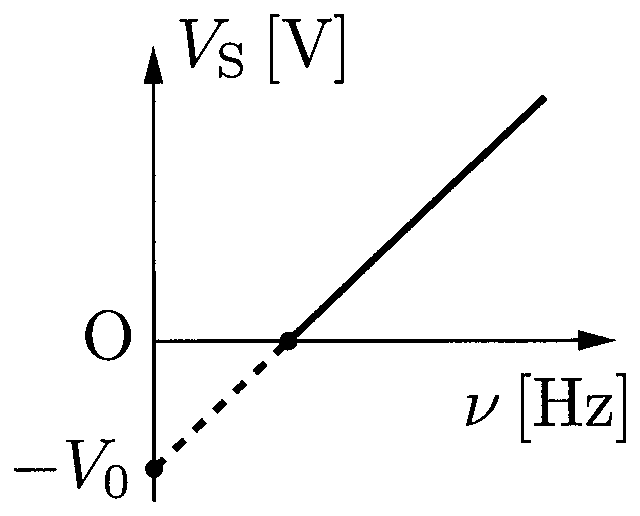
\includegraphics[keepaspectratio,width=30mm]{fig/n33_p4_zu3.png}\\
{\small\hspace{12mm}図2\hspace{26mm}図3}
\end{zuright}

\Mon[\Sitei]{コンプトン効果}

\begin{zuright}{56mm}
\hspace{1zw}波長の短いX線を物質に当てると，物質中の電子と衝突してX線は散乱されるが，散乱したX線の中には波長が変化したものが含まれることが知られており，これをコンプトン効果という．これについて考えてみよう．
\par
\hspace{1zw}今，図のように波長$\lambda\U{m}$のX線を，静止している電子に衝突させたところ，$90^\circ$ずれた方向で波長が$\lambda^\prime\U{m}$に変化した散乱X線が観測された．一方，この電子はX線の入射方向と角$\alpha$だけずれた方向に速さ$v\U{m/s}$ではね飛ばされた．
\zusep
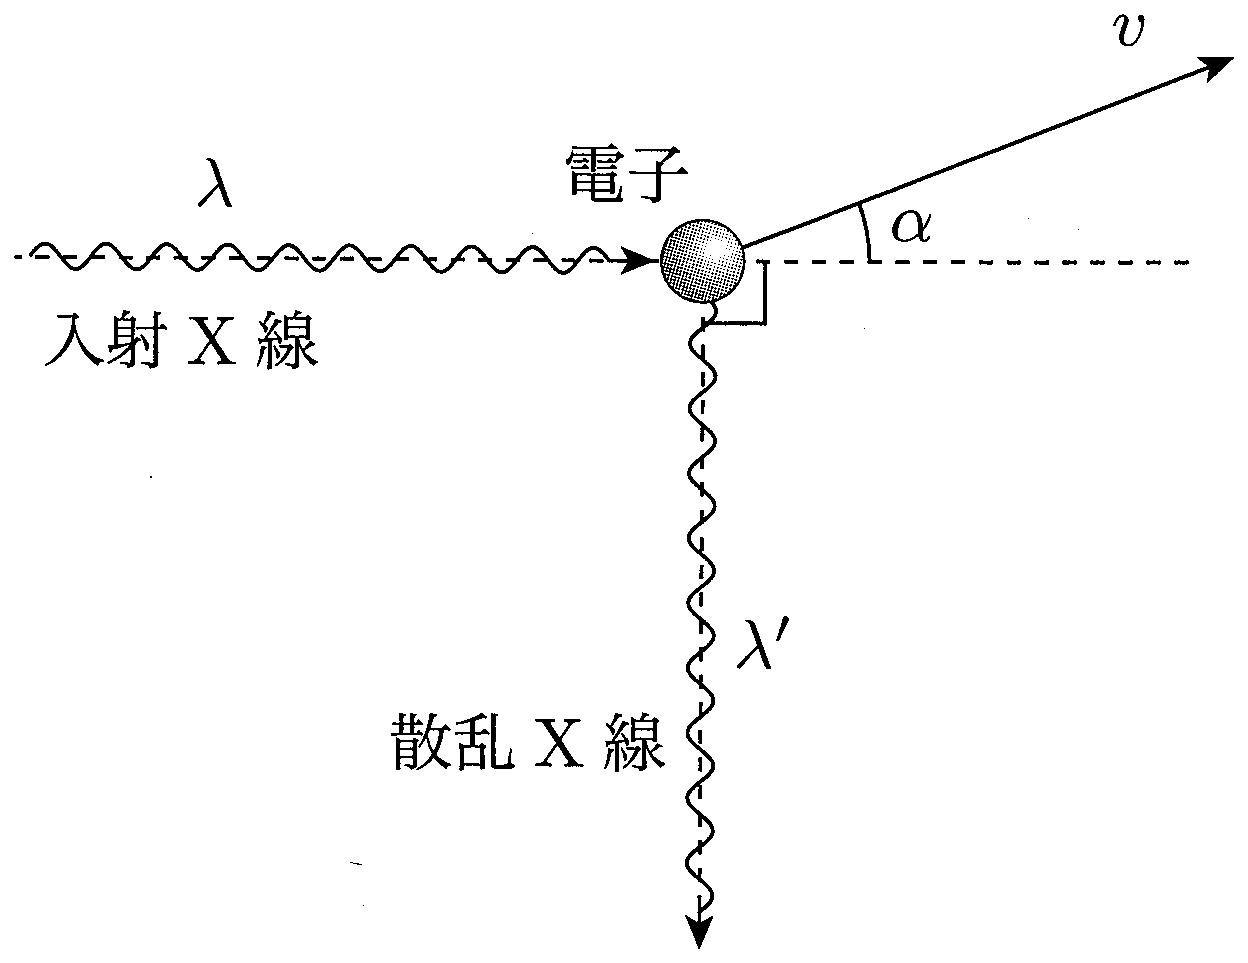
\includegraphics[keepaspectratio,width=54mm]{fig/n33_p5_zu.png}
\end{zuright}
\hspace{1zw}プランク定数，電子の質量，光速をそれぞれ$h\U{J\cdot s}$，$m\U{kg}$，$c\U{m/s}$とし，入射X線，散乱X線，および電子のはね飛ばされた方向はすべて同一平面内にあるものとして，以下の設問に答えよ．
\begin{komon}
\ko{1} $\lambda$，$\lambda^\prime$の大小関係を理由と共に答えよ．
\ko{2} 衝突の前後について成り立つエネルギー保存則および運動量保存則の式を示せ．
\ko{3} 実験により，光子の波長の変化$\Delta\lambda=\lambda^\prime-\lambda$は十分に小さく，$|\Delta\lambda|\ll\lambda$が満たされることが知られている．このとき，近似式$\dfrac{\lambda}{\lambda^\prime}+\dfrac{\lambda^\prime}{\lambda}\fallingdotseq 2$を用いて，散乱されたX線の波長$\lambda^\prime$を$\lambda$，$h$，$m$，$c$を用いて表せ．
\end{komon}

\Mon[\Sitei]{ボーアモデル}

\hspace{1zw}水素原子内の電子（質量$m\U{kg}$，電荷$-e\U{C}$）は半径$r\U{m}$，速さ$v\U{m/s}$で等速円運動をし，その軌道としては，円周に電子の定在波が生じているものだけが許され，陽子が電子に及ぼすクーロン力によって電子は等速円運動をしている．プランク定数を$h\U{J\cdot s}$，クーロンの法則の比例定数を$k\U{N\cdot m^2/C^2}$とする．電子のエネルギーは運動エネルギーとクーロン力による位置エネルギーとの和であり，クーロン力による位置エネルギーは無限遠方を基準点とする．以上のことを用いて，以下の設問に答えよ．ただし，水素原子における電子の基底状態のエネルギーは$E_1=-2.2\times 10^{-18}\U{J}$であり，$h=6.6\times 10^{-34}\U{J\cdot s}$，光速$c=3.0\times 10^8\U{m/s}$，電子の電荷$-e=-1.6\times 10^{-19}\U{C}$である．
\begin{komon}
\ko{1} 電子が量子数$n$の状態にあるときのエネルギー$E_n$を，$k$，$m$，$e$，$h$，$n$で表せ．また，$E_1$の値を$\U{eV}$単位で求めよ．
\ko{2} 電子が次に高いエネルギー状態にあるとき，そのエネルギー準位はいくらか．$\U{J}$単位で求めよ．
\ko{3} 基底状態にある電子に$7.0\times 10^{-19}\U{J}$のエネルギーを持つ光子を当てると，どのようなことが起こるか．
\ko{4} 量子数$n=3$の状態から$n=2$の状態に電子が移るときに放出される光の波長はいくらか．
\ko{5} 1価にイオン化したヘリウムイオン$\mathrm{He^+}$は，2個の陽子と2個の中性子とからなる原子核のまわりを1個の電子が等速円運動をしている．この電子の量子数$n$の軌道半径を与える式を，$k$，$m$，$e$，$h$，$n$で表せ．
\ko{6} $\mathrm{He^+}$の基底状態のエネルギーを$\U{J}$単位で求めよ．
\end{komon}

\Mon[\Sitei]{水素原子のスペクトル}

\hspace{1zw}以下の空欄\BOX{1}〜\BOX{7}に当てはまる，適当な語句または式を答えよ．
\par
\hspace{1zw}水素原子の放出する光のスペクトルの波長$\lambda\U{m}$は，
\[\frac{1}{\lambda}=R\Bigl(\frac{1}{m^2}-\frac{1}{n^2}\Bigr)\quad\cdots\cdots\text{\MARU{1}}\]
の形で表される．ここで$m$，$n$とは正の整数であり，$R$をリュードベリ定数という．
\par
\hspace{1zw}ボーアはこのスペクトルの規則性を説明するために，原子内の電子にはとびとびのエネルギー値（エネルギー準位）をもつ安定な軌道があり，電子がこのような安定な軌道の1つから他の安定な軌道へ移る（遷移する）ときには，2つの軌道のエネルギーの差を光子として\BOX{1}または\BOX{2}すると考えた．電子がエネルギー準位$E_n$から$E_m$へ遷移するとき（ただし$E_n>E_m$とする），プランク定数を$h\U{J\cdot s}$，\BOX{3}される光の振動数を$\nu\U{Hz}$とすると，
\[h\nu=\text{\BOX{4}}\quad\cdots\cdots\text{\MARU{2}}\]
の関係を満たすエネルギーをもつ光子が\BOX{3}される．ただし，ここで光速を$c\U{m/s}$とすれば，$c$，$\nu$，$\lambda$の間には\BOX{5}の関係が成り立つので，\MARU{2}とから，このとき放出される光の波長の逆数$\dfrac{1}{\lambda}$は，
\[\frac{1}{\lambda}=\text{\BOX{6}}\quad\cdots\cdots\text{\MARU{3}}\]
となる．\MARU{1}の$m$，$n$をそれぞれエネルギー準位の状態を示す数と考え，\MARU{1}\MARU{3}を比較すれば，$n$が無限大のとき（電子が原子核に対して無限遠方にあるとき）のエネルギー準位を$0\U{J}$とすると，水素原子内電子のエネルギー準位$E_n$の一般式は，
\[E_n=\text{\BOX{7}}\]
で与えられる．

\filbreak
\Rank{C問題}

\Mon{光電管とコンデンサー}

\begin{zuright}{46mm}
\hspace{1zw}図1のような光電管，電気容量$C=5.0\U{\mu F}$のコンデンサー$\mathrm{C}$，抵抗値$R=2.0\U{M\Omega}$の抵抗$\mathrm{R}$を含む回路がある．$\mathrm{PQ}$間の電圧を$v\U{V}$，電流計を流れる電流を$i\U{A}$とする．$v=0\U{V}$の状態から，スイッチ$\mathrm{S}$を開いたまま光電管の陰極$\mathrm{K}$に波長$\lambda_1=0.50\U{\mu m}$の光を一定の強度で照射し続けたところ，回路にしばらくの間電流が流れ，やがて止まった．その間の$v$と$i$を測定したところ，図2の実線で示す直線が得られた．これがこの光電管の電流－電圧特性曲線を示すものとして，以下の設問に答えよ．ただし電気素量$e=1.6\times 10^{-19}\U{C}$，光の速さを$c=3.0\times 10^8\U{m/s}$とする．
\begin{komon}
\ko{1} 波長$\lambda_1$の光の照射により陰極$\mathrm{K}$から飛び出す電子の運動エネルギーの最大値$K_{\max 1}\U{J}$はいくらか．
\ko{2} 回路に電流が流れなくなったとき，コンデンサーに蓄えられている電気量$Q_0\U{C}$を求めよ．
\ko{3} 光を照射し続けたままスイッチ$\mathrm{S}$を閉じると，しばらくして回路に一定の電流$i_0\U{A}$が流れるようになった．この電流量$i_0$を求めよ．
\ko{4} 光の照射をやめ，$\mathrm{PQ}$間の電圧を$v=0\U{V}$に戻したのち，再びスイッチ$\mathrm{S}$を開き，$\lambda_1$と異なる波長$\lambda_2=0.75\U{\mu m}$の光を一定の強度で照射し続けたところ，$\mathrm{PQ}$間の電圧$v$が$1.0\U{V}$となったとき，回路に流れる電流が$i=0\U{A}$となった．以上の測定結果を用いて，プランク定数$h\U{J\cdot s}$の値を計算せよ．
\end{komon}
\zusep
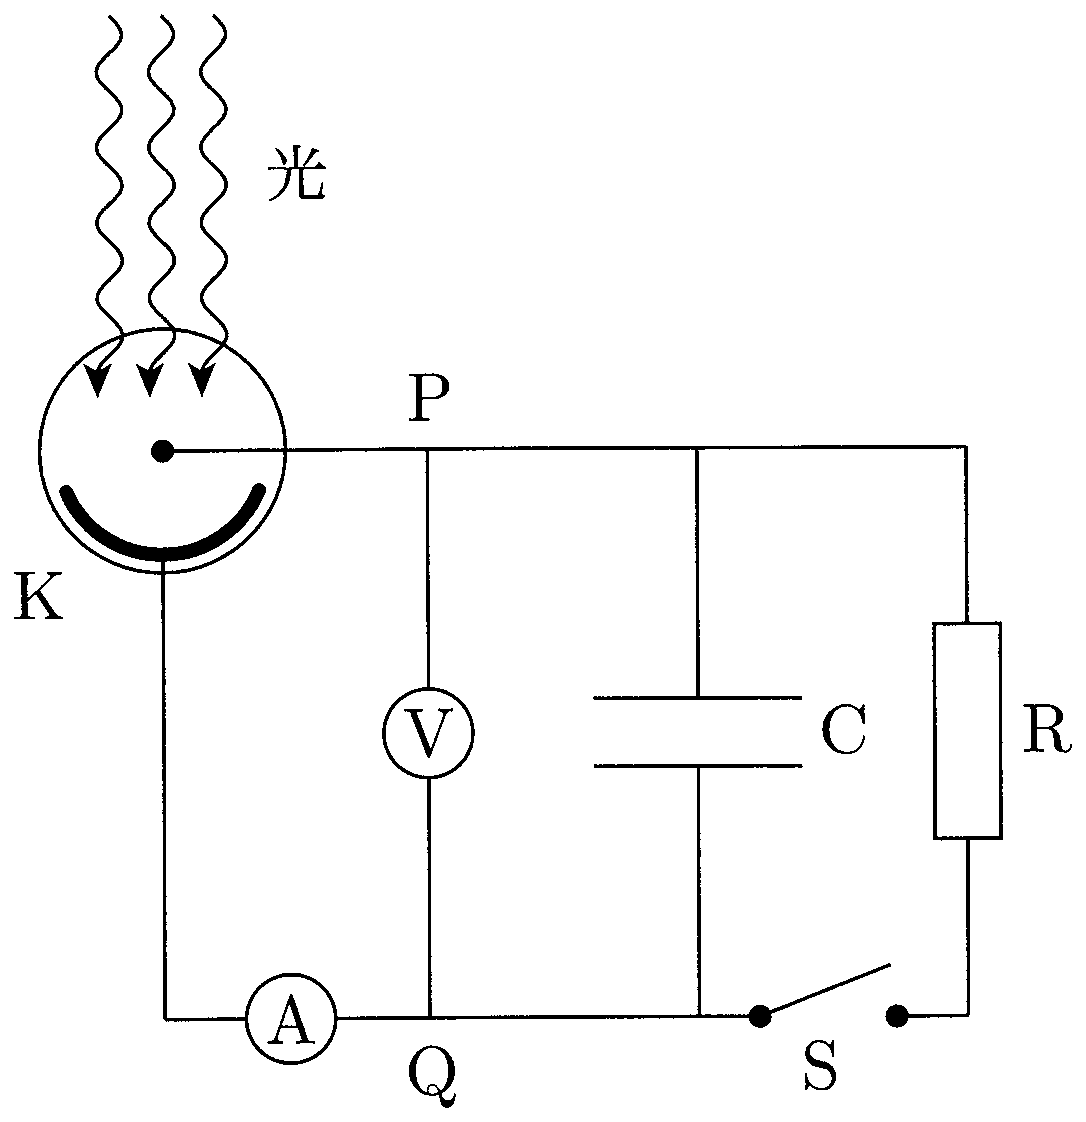
\includegraphics[keepaspectratio,width=40mm]{fig/n33_p8_zu1.png}\\{\small 図1}\\[2mm]
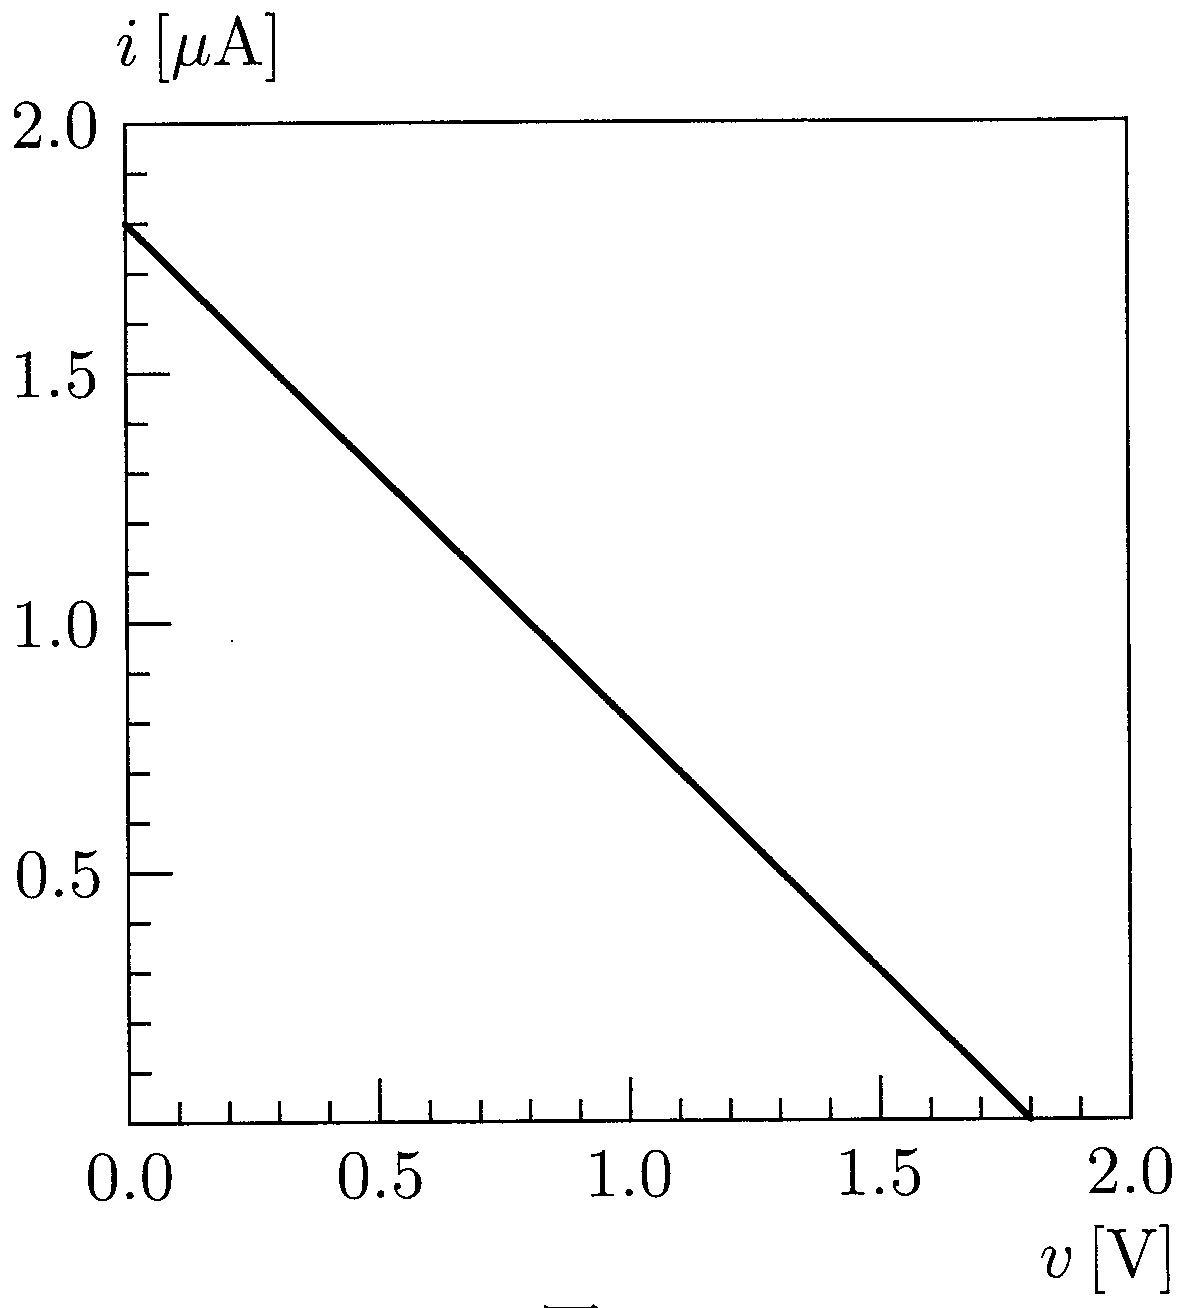
\includegraphics[keepaspectratio,width=44mm]{fig/n33_p8_zu2.png}\\{\small 図2}
\end{zuright}

\Mon{フランク・ヘルツの実験}

\begin{zuright}{50mm}
\hspace{1zw}図1において$\mathrm{F}$はフィラメント，$\mathrm{P}$は電位$0\U{V}$の電極，$\mathrm{G}$はグリッドである．$\mathrm{G}$はいつも小さい正の電位（$0.5\U{V}$）に保たれており，$\mathrm{F}$の電位$-V\U{V}$は$0\U{V}$から約$-100\U{V}$程度まで変えられるようになっている．ここで容器の中に低圧の水銀蒸気を入れた後，$V$を変化させて検流計$\mathrm{A}$を流れる電流$i\U{A}$を測定したところ，図2のようなグラフが得られた．以下の設問に答えよ．
\zusep
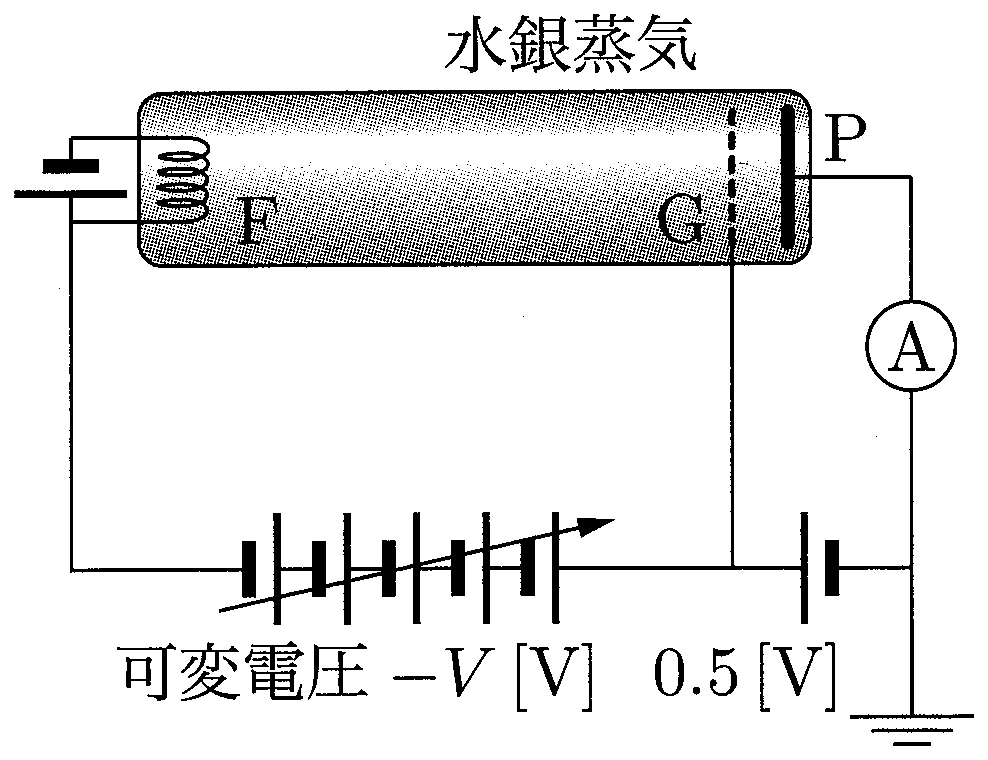
\includegraphics[keepaspectratio,width=44mm]{fig/n33_p9_zu1.png}\\{\small 図1}\\[1mm]
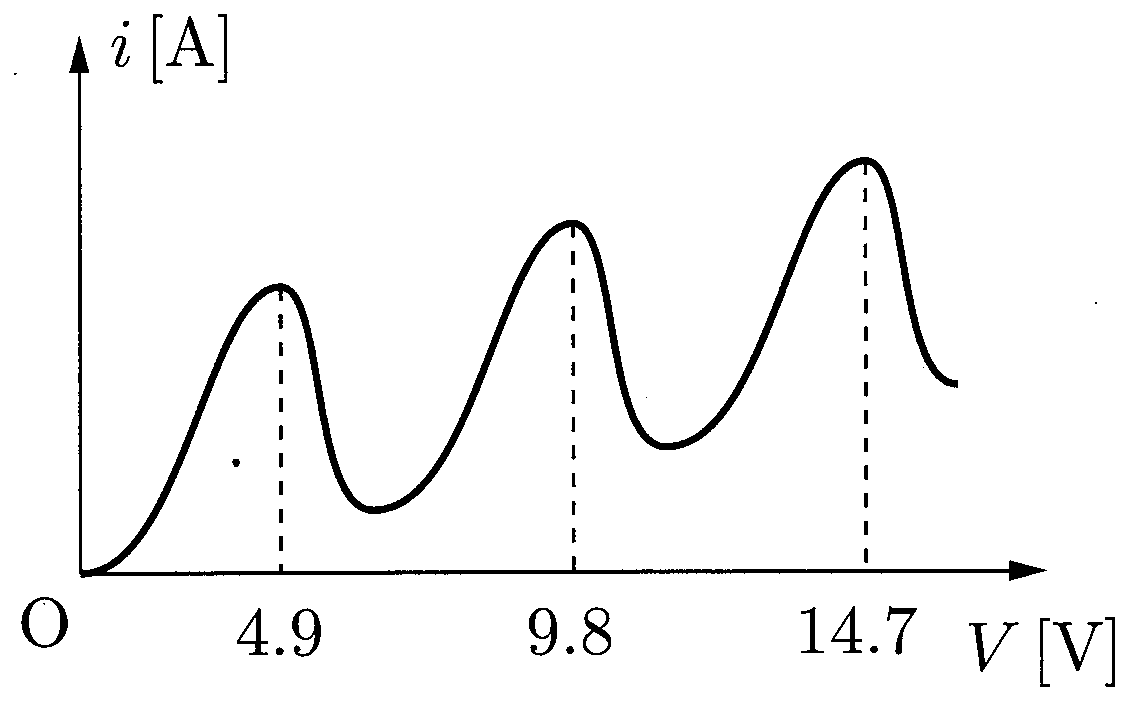
\includegraphics[keepaspectratio,width=46mm]{fig/n33_p9_zu2.png}\\{\small 図2}
\end{zuright}
\begin{komon}
\ko{1} 次の文中の空欄\BOX{ア}〜\BOX{キ}に適当な語句および式を埋めよ．
 \begin{description}
 \item[\MARU{1}] $\mathrm{F}$からは電子が放射され，電子は$\mathrm{FG}$間で\BOX{ア}される．
 \item[\MARU{2}] 電子は$\mathrm{P}$に達するまでに水銀原子と衝突するが，運動エネルギーが小さい場合は原子と衝突しても，エネルギーは失われない．すなわち電子と原子との衝突は\BOX{イ}である．
 \item[\MARU{3}] 運動エネルギーがある値$E\U{J}$を越えると，衝突の際原子にエネルギーを与えて，この原子を低いエネルギーの状態（エネルギー準位$E_1\U{J}$）から，高いエネルギーの状態（エネルギー準位$E_2\U{J}$）に励起する．この$E$は$E_1$，$E_2$を用いて，$E=$\BOX{ウ}と表せる．またこのときの電子と原子との衝突は\BOX{エ}である．
 \item[\MARU{4}] 電子は$\mathrm{GP}$間では\BOX{オ}されるので，十分エネルギーを持っていなければ，$\mathrm{P}$に達することができず，$\mathrm{G}$に捕らえられてしまう．
 \item[\MARU{5}] 電流$i$は$\mathrm{G}$を通り抜けて$\mathrm{P}$に達しうる電子の数が\BOX{カ}ほど，また電子の速さが\BOX{キ}ほど，大きくなる．
 \end{description}
\ko{2} 次の文中の空欄\BOX{ク}〜\BOX{コ}に相当する説明を(1)の\MARU{1}〜\MARU{5}の中から選べ．
 \begin{description}
 \item[・] $V$が$4.9\U{V}$を越えると$i$が急に減少するのは，\BOX{ク}の過程によってエネルギーを失った電子が\BOX{ケ}のために$\mathrm{P}$に到達できなくなるためである．
 \item[・] $V$をさらに大きくすると，$i$は再び増加するが，$V$が$9.8\U{V}$を越えるとまた減少する．これは最初の衝突でエネルギーを失った電子が，$V$が十分大きいために$\mathrm{P}$に達するまでにもう一度加速され，\BOX{コ}の過程を引き起こすからだと考えられる．
 \end{description}
\end{komon}

\newpage

%%%%%%%%%%%%%%%%%%%%  解答  %%%%%%%%%%%%%%%%%%%%
\KaiTitle{第33回　光の粒子性・物質波と原子模型}
\setlength{\columnseprule}{0.4pt}
\begin{multicols}{2}
\raggedcolumns

\Rank{A問題}
\MonN{1}{基本事項の確認}\par\nopagebreak
\begin{sisin}
光子のエネルギー，運動量の大きさの式$\varepsilon=h\nu$，$p=\dfrac{h}{\lambda}$の2つをしっかりと覚えておくこと．光子のエネルギーの式は波長を使って書くと$\varepsilon=\dfrac{hc}{\lambda}$と書き換えられるが，この式から分かるように，{\gtfamily 波長が短いほど光子のエネルギーは大きい}．このことは常識として覚えておくこと．色と波長の関係は長波長側から「赤，橙，黄，緑，青，藍，紫」，可視光の波長領域は$380\sim 780\U{nm}$程度であることも再度確認しておくこと．
光子の振動数は一般に$f$ではなく$\nu$（ニュー）と書く．$v$（ヴイ）との書き分けをきっちり行うこと．
ミリカンの実験の値から電気素量を求める場合は，例題1と同じく，まず小さい方から順に並べて差を取り，おおざっぱな値から各電荷が電気素量何個分かを求める．
物質波の波長の式$\lambda=\dfrac{h}{mv}$は，光子の運動量$p=\dfrac{h}{\lambda}$と対比させて覚えておくとよい．
ラザフォードの実験については，\MARU{1}どのような実験をして，\MARU{2}どのような結論を導いたのか，の概要を覚えておくとよい（33.6）．
\end{sisin}
\KaiHead
\begin{komon}
\ko{1} エネルギー保存則より$\dfrac{1}{2}m_ev^2=eV$．よって
       \[v=\sqrt{\frac{2eV}{m_e}}\fallingdotseq 8.4\times 10^6\U{m/s}\Ans\]
\ko{2} 小さい方から並べて差を取ると$3.19$，$1.62$，$1.58$，$4.77$であるから，帯電量はおよそ$1.6\times 10^{-19}\U{C}$の整数倍になっていると考えられる．よって各帯電量は$4.86\fallingdotseq 3e$，$8.05\fallingdotseq 5e$，$9.67\fallingdotseq 6e$，$11.25\fallingdotseq 7e$，$16.02\fallingdotseq 10e$と考えられる（$3+5+6+7+10=31$個分）．以上より
       \[\begin{aligned}e&=\frac{4.86+8.05+9.67+11.25+16.02}{31}\\&\qquad\times 10^{-19}\\&\fallingdotseq 1.61\times 10^{-19}\U{C}\end{aligned}\]
       \hspace*{\fill}$\cdots$(答)
\ko{3} \[\begin{aligned}E&=\frac{hc}{\lambda}=\frac{6.63\times 10^{-34}\times 3.0\times 10^8}{6.0\times 10^{-7}}\\&\fallingdotseq 3.3\times 10^{-19}\U{J}\end{aligned}\]
       \hspace*{\fill}$\cdots$(答)
       \[\begin{aligned}p&=\frac{h}{\lambda}=\frac{6.63\times 10^{-34}}{6.0\times 10^{-7}}\\&\fallingdotseq 1.1\times 10^{-27}\U{kg\cdot m/s}\end{aligned}\]
       \hspace*{\fill}$\cdots$(答)
\ko{4} 限界振動数の光子を当てたときにぎりぎり電子が飛び出すので，$h\nu_0=0+W$．よって
       \[W=6.63\times 10^{-34}\times 3.3\times 10^{14}\fallingdotseq 2.2\times 10^{-19}\U{J}\]
       \hspace*{\fill}$\cdots$(答)
\ko{5} 各色の波長はおおよそ，紫（$400\U{nm}$）$<$緑（$500\U{nm}$）$<$赤（$700\U{nm}$）程度である．限界の光が緑であるということは，これより高いエネルギーを持つ（波長の短い）光子でしか光電効果を起こせない．よって\\
       \hspace*{\fill}赤色：飛び出さない\quad 紫色：飛び出す\Ans
\ko{6} $h\nu_0=W$，$h\nu=\dfrac{1}{2}m_ev_{\max}^2+W$より$\dfrac{1}{2}m_ev_{\max}^2=h(\nu-\nu_0)$．これを解いて
       \[v_{\max}=\sqrt{\frac{2h(\nu-\nu_0)}{m_e}}\fallingdotseq 5.0\times 10^5\U{m/s}\]
       \hspace*{\fill}$\cdots$(答)
\ko{7} 粒子性：光電効果，コンプトン効果\quad 波動性：干渉，回折\Ans
\ko{8} \[\begin{aligned}\lambda&=\frac{h}{m_ev}=\frac{6.63\times 10^{-34}}{9.1\times 10^{-31}\times 1.0\times 10^7}\\&\fallingdotseq 7.3\times 10^{-11}\U{m}\end{aligned}\]
       \hspace*{\fill}$\cdots$(答)
\ko{9} \MARU{1}\ 原子の中心に，原子のほぼ全質量を持つ原子核が存在する．\MARU{2}\ 原子番号$Z$の原子核は$+Ze$の正電荷を持っている．また，原子核の半径は電子の円運動半径に比べて非常に小さい．\MARU{3}\ 原子核の周囲を$Z$個の電子が回っており，原子核の正電荷を中和して電気的に中性になっている．\Ans
\ko{10} 電子が失ったエネルギー分の光子が放出されるので
       \[\begin{aligned}h\nu&=-0.85-(-3.40)=2.55\U{eV}\\&=2.55\times 1.6\times 10^{-19}\fallingdotseq 4.1\times 10^{-19}\U{J}\end{aligned}\]
       \hspace*{\fill}$\cdots$(答)
       \[\nu=\frac{4.08\times 10^{-19}}{6.63\times 10^{-34}}\fallingdotseq 6.2\times 10^{14}\U{Hz}\Ans\]
\end{komon}

\Rank{B問題}
\MonN[\Sitei]{2}{ミリカンの実験}\par\nopagebreak
\begin{sisin}
実際にミリカンの行った実験は，講義（33.1）で述べたように空気の粘性抵抗を考えるなど複雑な式を利用した精密なものであるが，これを簡素化して考えさせたものが本問である．油滴に作用する力，すなわち重力，空気からの抵抗力，電場からのクーロン力（静電気力）の3つの力を押さえ，力のつり合いの式から条件を定めていこう．なお，当然のことだが空気からの抵抗力は油滴の移動方向と逆向きにかかることに注意．
\end{sisin}
\KaiHead
\begin{komon}
\ko{1} 油滴が速さ$v$で下降するとき，油滴には上向きに大きさ$kv$の空気抵抗が作用する．重力によって速さが増すにつれて抵抗力が増加し，ついに2つの力がつり合うとそれ以上速さが増加しなくなる．よって終端速度に達したときには力がつり合っており，
       \[kv_0=mg\quad\Leftrightarrow\quad v_0=\frac{mg}{k}\U{m/s}\Ans\]
\ko{2} この油滴は電場から上向きに$qE\U{N}$の力を受けるので，$qE=mg$が満たされ，なおかつ速度が$0$となればそのまま静止しつづけることができる．ゆえに
       \[E_0=\frac{mg}{q}\U{N/C}\Ans\]
\ko{3} 2つの式から油滴の質量$m$（小さすぎるので測定できない）を消去すると，
       \[q=\frac{kv_0}{E_0}\U{C}\Ans\]
\end{komon}

\MonN[\Sitei]{3}{光電効果}\par\nopagebreak
\begin{sisin}
光電効果に関するまとめの問題である．光電効果の特徴はこの問題にほぼすべてまとめられているので，本問をしっかりと押さえておこう．
飛び出す電子の持つ運動エネルギーが$h\nu-W$であると勘違いしやすいので注意せよ．飛び出す電子はさまざまな運動エネルギーを持つが，その{\gtfamily 最大値}が$h\nu-W$である．
A問題の指針でも述べたが，光子のエネルギーは振動数が大きいほど，波長が短いほど大きいということを忘れないように．(15)(17)は不等式で考えていけば明らかであるが，以上なのか以下なのかは不等式を考えなくてもすぐに判断できるようにしておくこと．
\end{sisin}
\KaiHead
\begin{komon}
\ko{1} は持たないが\Ans
\ko{2} 光子（光量子）\Ans
\item[{\makebox[1.9zw][r]{(3)(4)}}] 回折，干渉（順不同）\Ans
\ko{5} 波動\Ans
\ko{6} $h\nu$\Ans
\ko{7} $p=\dfrac{h}{\lambda}$ゆえ，$\dfrac{h\nu}{c}$\Ans
\ko{8} 光電子\Ans
\ko{9} はない\Ans
\ko{10} 最小\Ans
\ko{11} 仕事関数\Ans
\ko{12} よって異なる\Ans\par
       （電子の取り出しやすさは金属ごとに異なる．イオン化エネルギーが原子ごとに違うのと同様．）
\ko{13} 金属表面から電子が飛び出したときが最も電子の飛び出しに必要なエネルギーが少なくて済み，そのため飛び出した電子の運動エネルギーが最大になる．このときのエネルギー保存則は$h\nu=K_{\max}+W$であり，
       \[K_{\max}=h\nu-W\Ans\]
\item[{\makebox[1.9zw][r]{(14)(15)}}] 表面から電子を取り出すのが最も容易で，これには$W$のエネルギーが必要であるが，光子のエネルギーが$W$未満だと表面からすら電子を取り出せないことになり，光電効果は起こらない．よって$h\nu\geqq W$，すなわち光の振動数は
       \[\frac{W}{h}\ \text{以上}\Ans\]
\item[{\makebox[1.9zw][r]{(16)(17)}}] 光電効果が起こるためには$\dfrac{hc}{\lambda}\geqq W$であることが必要である．これより，光の波長は
       \[\frac{hc}{W}\ \text{以下}\Ans\]
\ko{18} 限界振動数\Ans
\ko{19} 限界波長\Ans
\end{komon}

\MonN[\Sitei]{4}{光電管}\par\nopagebreak
\begin{sisin}
光電管の使い方，グラフの読み取り方などに関する総合問題であるが，数式だけで追いかけようとすると分からなくなる．光子によってはじき出された電子がそのあとどのように動いていくのかを頭でイメージしながら考えれば分かりやすいだろう（33.3）．
\end{sisin}
\KaiHead
\begin{komon}
\ko{1} 光子が陰極板$\mathrm{C}$にぶつかると光電効果により電子がはじき出されるが，これが向かい側の陽極板に到達すると電流計や抵抗を通過して再び$\mathrm{C}$へと戻る．よって，電子は電流計をア$\to$イの向きに通過する．電流の向きと電子の移動方向とは逆なので，電流の向きは
       \[\text{イ}\to\text{ア}\Ans\]
\ko{2} 電流が飽和するのは，極板$\mathrm{C}$において発生した光電子がすべて向かい合う陽極板へと吸い込まれているからである．この飽和電流が$I_0$であるということは，単位時間（1秒）あたりに陽極に入ってくる電子の数が$\dfrac{I_0}{e}$個であるということを意味する．ゆえに，陰極板から単位時間あたりに出てくる光電子の数は
       \[\frac{I_0}{e}\ \text{個}\Ans\]
\ko{3} 阻止電圧が$-V_{\mathrm{S}}$であるということは，陰極$\mathrm{C}$に対して陽極を$-V_{\mathrm{S}}$にすると，最大の運動エネルギーを持つ電子すらも陽極に達することができないということを意味する．よって$\dfrac{1}{2}mv_{\max}^2=eV_{\mathrm{S}}$．これを解いて
       \[v_{\max}=\sqrt{\frac{2eV_{\mathrm{S}}}{m}}\U{m/s}\Ans\]
\ko{4} 光の振動数が$\nu$のときに出てくる電子の最大運動エネルギー$K_{\max}$は，陰極板$\mathrm{C}$の仕事関数を$W$として，$h\nu=K_{\max}+W$である．また$K_{\max}=eV_{\mathrm{S}}$の関係があるので
       \[V_{\mathrm{S}}=\frac{h}{e}\nu-\frac{W}{e}\]
       よって，これをグラフ化した場合の傾きは
       \[\frac{h}{e}\U{V/Hz}\Ans\]
\ko{5} グラフの切片は，上の式より$-V_0=-\dfrac{W}{e}$であるから$eV_0=W$．すなわち，$eV_0$の値は{\gtfamily 陰極板$\mathrm{C}$の仕事関数}を表す．\Ans
\ko{6} (4)の式で$V_{\mathrm{S}}=0$とおくと$h\nu=W$であり，このとき$K_{\max}=0$である．つまり，これは電子がぎりぎり飛び出す場合を表している．すなわち，グラフの$\nu$軸切片は{\gtfamily 限界振動数}を表す．\Ans
\end{komon}

\MonN[\Sitei]{5}{コンプトン効果}\par\nopagebreak
\begin{sisin}
コンプトン効果を扱う問題は，ほぼ講義の例題4のみですべてカタがつくので，まずはしっかりと例題を押さえておくこと．本問は，散乱角が$90^\circ$の場合に特化して考えさせる問題であるが，指針は例題4と全く同じ．運動量保存則とエネルギー保存則の二つの式を組み合わせて考えよう．二つの式から文字を消去する手順を間違えないように注意せよ．
(1)については，(2)のエネルギー保存則の式からも判断できるが，解答に示した考え方で一瞬で判断できるようにしておくこと．
% 原本は「テキストの例題」．例題4（原本の例題4）を指す．
\end{sisin}
\KaiHead
\begin{komon}
\ko{1} 光子（X線）のエネルギーの一部が電子の運動エネルギーに転化したので，散乱X線のエネルギーは入射X線のエネルギーに比べて小さい．光子は波長が長いほどエネルギーが小さいので，波長の大小関係は
       \[\lambda^\prime>\lambda\Ans\]
\ko{2} エネルギー保存則の式は
       \[\frac{hc}{\lambda}=\frac{1}{2}mv^2+\frac{hc}{\lambda^\prime}\Ans\]
       運動量保存則の式は
       \[\text{入射方向：}\ \frac{h}{\lambda}=mv\cos\alpha\]
       \[\text{垂直な方向：}\ 0=mv\sin\alpha-\frac{h}{\lambda^\prime}\Ans\]
       もしくは，下図の運動量保存則の関係を表すベクトル図に対する三平方の定理より
       \begin{center}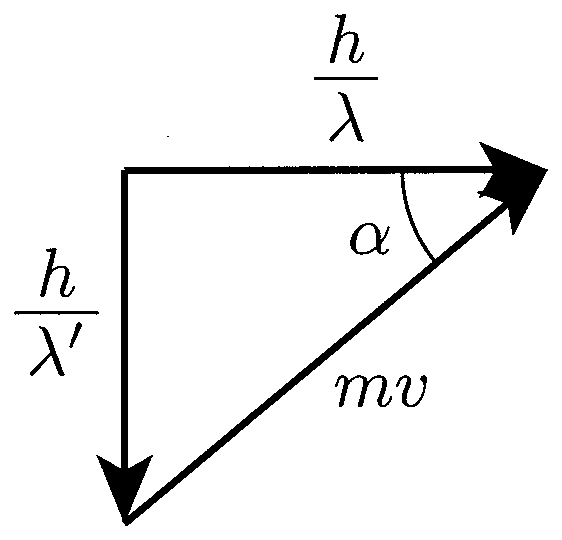
\includegraphics[keepaspectratio,width=26mm]{fig/n33_a5_vec.png}\end{center}
       \[\Bigl(\frac{h}{\lambda^\prime}\Bigr)^2+\Bigl(\frac{h}{\lambda}\Bigr)^2=(mv)^2\Ans\]
       \begin{bsHosoku}{参考}
       最後の関係式は，軸方向を分けて立てた式から$\alpha$を消去して得られる．なお，このベクトル図に対して立てるべき式は，角度$\alpha$に対しての余弦定理ではなく，直角に対しての三平方の定理である（(3)で最終的に求めるのは，$\alpha$を含まない形の答であるから）．
       \end{bsHosoku}
\ko{3} エネルギー保存則の式を変形して$m^2v^2=\dfrac{2mhc}{\lambda}-\dfrac{2mhc}{\lambda^\prime}$であるから，
       \[\Bigl(\frac{h}{\lambda^\prime}\Bigr)^2+\Bigl(\frac{h}{\lambda}\Bigr)^2=\frac{2mhc}{\lambda}-\frac{2mhc}{\lambda^\prime}\]
       が成立する．両辺に$\lambda\lambda^\prime$をかけると
       \[h^2\Bigl(\frac{\lambda}{\lambda^\prime}+\frac{\lambda^\prime}{\lambda}\Bigr)=2mhc(\lambda^\prime-\lambda)\]
       近似式$\dfrac{\lambda}{\lambda^\prime}+\dfrac{\lambda^\prime}{\lambda}\fallingdotseq 2$を用いると$2h^2\fallingdotseq 2mhc(\lambda^\prime-\lambda)$となるので，これを解いて
       \[\lambda^\prime=\lambda+\frac{h}{mc}\U{m}\Ans\]
       \begin{bsHosoku}{参考}
       $\dfrac{h}{mc}\fallingdotseq 2.43\times 10^{-12}\U{m}$のことをコンプトン波長といい，コンプトン効果による光の波長のずれの目安として用いる．値から分かるように，コンプトン効果による波長のずれというのは，X線のような短い波長の電磁波でなければ観測できないほど小さいものである．
       \end{bsHosoku}
\end{komon}

\MonN[\Sitei]{6}{ボーアモデル}\par\nopagebreak
\begin{sisin}
ボーアモデルに関する総合問題である．まず，誘導なしで(1)の，水素原子のエネルギー準位の式を導けるようにせよ．立てるべき式は，\MARU{1}運動方程式，\MARU{2}量子条件の式，\MARU{3}力学的エネルギーの式，の3つである（例題6）．変形の仕方にもコツがあるので，そこまできっちり覚えておくこと．
また，結果として得られる水素原子のエネルギー準位の式の$E_1$の値（$-13.6\U{eV}$）は覚えておくこと．
ヘリウムイオンについてだが，電子が1つだけ，ということは，\MARU{1}〜\MARU{3}式が若干変わるだけで，水素原子の場合とほぼ同様である．\MARU{1}〜\MARU{3}の式をどのように変えればいいのかを考えて処理せよ．
\end{sisin}
\KaiHead
\begin{komon}
\ko{1} 水素原子内における電子の半径方向の運動方程式は
       \[m\frac{v^2}{r}=k\frac{e^2}{r^2}\quad\cdots\text{\MARU{1}}\]
       また，電子のド・ブロイ波長は$\lambda=\dfrac{h}{mv}$であるから，量子条件は
       \[2\pi r=n\frac{h}{mv}\quad\cdots\text{\MARU{2}}\]
       このとき電子の持つ力学的エネルギーは
       \[E_n=\frac{1}{2}mv^2-k\frac{e^2}{r}\quad\cdots\text{\MARU{3}}\]
       である．\MARU{1}より$mv^2=k\dfrac{e^2}{r}$，\MARU{2}より$mv=\dfrac{nh}{2\pi r}$であるから，この2つの式から$v$を消去して
       \[r=\frac{n^2h^2}{4\pi^2mke^2}\]
       \MARU{1}と\MARU{3}から$v$を消去すると$E_n=-\dfrac{1}{2}k\dfrac{e^2}{r}$であり，これに$r$を代入して
       \[E_n=-\frac{2\pi^2mk^2e^4}{h^2}\cdot\frac{1}{n^2}\U{J}\Ans\]
       また，$E_1=-2.2\times 10^{-18}\U{J}$を$\U{eV}$単位に換算すると
       \[-\frac{2.2\times 10^{-18}}{1.6\times 10^{-19}}\fallingdotseq -14\U{eV}\Ans\]
\ko{2} 次に高いエネルギー状態とは，$n=2$の状態である．(1)より
       \[E_2=\frac{E_1}{4}=-5.5\times 10^{-19}\U{J}\Ans\]
\ko{3} 基底状態にある電子がこの光子を吸収したとすると，$E_1+7.0\times 10^{-19}=-1.5\times 10^{-18}\U{J}$のエネルギー状態へと遷移することになるが，そこにエネルギー準位が存在しなければ遷移先が存在しないため，電子はこの光子を吸収することができない．$\dfrac{E_1}{n^2}=-1.5\times 10^{-18}$とおくと$n^2\fallingdotseq 1.5$となり，$n$は整数でないので，この位置にエネルギー準位は存在しない．よって，{\gtfamily 光子は吸収されずにそのまま散乱される（通り過ぎる）}．\Ans
       \begin{bekkai}
       勘がよければ(2)の答えから考えてしまってもよい．基底状態から次の励起状態へ遷移するために必要なエネルギーは$E_2-E_1=1.65\times 10^{-18}\U{J}$であるが，$7.0\times 10^{-19}\U{J}$はこれより小さいので，基底状態のすぐ上の励起状態にすら電子を励起することができない．
       \end{bekkai}
\ko{4} $n=3$から$n=2$への遷移により失われる電子のエネルギーは
       \[E_3-E_2=\Bigl(\frac{1}{3^2}-\frac{1}{2^2}\Bigr)E_1\fallingdotseq 3.05\times 10^{-19}\U{J}\]
       であり，これだけのエネルギーを持つ光子が放出される．$\dfrac{hc}{\lambda}=3.05\times 10^{-19}$より
       \[\lambda\fallingdotseq 6.5\times 10^{-7}\U{m}\Ans\]
\ko{5} $\mathrm{He^+}$は，電荷$+2e$の原子核のまわりを1個の電子が等速円運動をしている．よって
       \[m\frac{v^2}{r}=k\frac{e\cdot 2e}{r^2}\quad\cdots\text{\MARU{4}}\]
       \[2\pi r=n\frac{h}{mv}\quad\cdots\text{\MARU{5}}\]
       \[E_n^\prime=\frac{1}{2}mv^2-k\frac{e\cdot 2e}{r}\quad\cdots\text{\MARU{6}}\]
       以上を整理して
       \[r=\frac{n^2h^2}{8\pi^2mke^2}\U{m}\Ans\]
\ko{6} 同様に$E_n^\prime=-\dfrac{8\pi^2mk^2e^4}{h^2}\cdot\dfrac{1}{n^2}$であり，基底状態のエネルギーは水素原子の場合の4倍になっているので
       \[E_1^\prime=4E_1=-8.8\times 10^{-18}\U{J}\Ans\]
       \begin{chuu}
       \MARU{4}〜\MARU{6}式はまともに計算する必要はない．これらの式は（形の上において）\MARU{1}〜\MARU{3}式において$k$を$2k$に取り替えたのと同じであるから，(1)で得られた答えについて，$k$を$2k$に取り替えたものが(5)(6)の答えである．
       \end{chuu}
\end{komon}

\MonN[\Sitei]{7}{水素原子のスペクトル}\par\nopagebreak
\begin{sisin}
振動数条件と呼ばれるエネルギー保存則に関する問題である．誘導に従って答えていけば特に難しい問題ではなかろう．なお，歴史的には水素原子の放出する光の分析から\MARU{1}式の関係が見い出されたため，これを説明するために水素原子に関するモデルなどが提唱されたが，なぜ\MARU{1}式のようになるのかは，水素原子のエネルギー準位の式から求めてみる（本問を逆に後ろから追いかける，33.6）と分かりやすいだろう．
\end{sisin}
\KaiHead
\begin{komon}
\item[{\makebox[1.9zw][r]{(1)(2)}}] 吸収，放出\Ans
\ko{3} 高エネルギー状態から低エネルギー状態への遷移であるから，余ったエネルギーが放出される．よって\quad 放出\Ans
\ko{4} 差分のエネルギーが放出されるので\quad $h\nu=E_n-E_m$\Ans
\ko{5} $c=\nu\lambda$\Ans
\ko{6} 2つの式を変形して
       \[\frac{1}{\lambda}=\frac{\nu}{c}=\frac{1}{ch}(E_n-E_m)\Ans\]
\ko{7} $\dfrac{1}{\lambda}=-\dfrac{1}{ch}(E_m-E_n)$であるから，これと\MARU{1}式との比較により
       \[-\frac{1}{ch}E_n=\frac{R}{n^2}+C\quad\text{（$C$は定数）}\]
       であることが分かる．ここで，$n\to\infty$のとき$E_n\to 0$となるように定数を決めると$C=0$であるから
       \[E_n=-\frac{chR}{n^2}\U{J}\Ans\]
       \begin{chuu}
       一見すると，比較によりいきなり$E_n=-\dfrac{chR}{n^2}$としたくなるだろうが，$E_n$に定数項がついていても$\dfrac{1}{\lambda}=-\dfrac{1}{ch}(E_m-E_n)$の関係を満たせることに注意せよ．
       \end{chuu}
\end{komon}

\Rank{C問題}
\MonN{8}{光電管とコンデンサー}\par\nopagebreak
\begin{sisin}
まずは電子の動きをしっかり押さえて，回路にどのように電圧がかかっていくのかを押さえよう．スイッチ$\mathrm{S}$を開いた状態では，コンデンサーに電子が流れ込んで電荷が溜まり，コンデンサーに電圧がかかる．コンデンサーに電圧がかかれば，光電管の陽極－陰極間に同じ電圧がかかることになり，それだけ電流が流れにくくなり，電流が減少していく．これが図2のグラフである．
また，問題文には全く「仕事関数」について触れられていないが，当然のことながら陰極$\mathrm{K}$には必ず仕事関数が存在する．よって，(1)のような問題であれば，まず仕事関数を適当な文字で置いて，光子のエネルギー，光電子の最大運動エネルギー，仕事関数の間に成立する関係式を立式することから始めよ．
\end{sisin}
\KaiHead
スイッチ$\mathrm{S}$を開いたままの状態で陰極$\mathrm{K}$に光を照射した場合について考える．発生した光電子はその後，陽極に入って$\mathrm{P}$点を通過してコンデンサー$\mathrm{C}$の上側極板へと到達する．コンデンサーの向かい合う極板には正負逆の電荷が帯電するため，コンデンサー$\mathrm{C}$の下側極板からは電子が$\mathrm{Q}\to\mathrm{K}$へと移動していく．
\begin{center}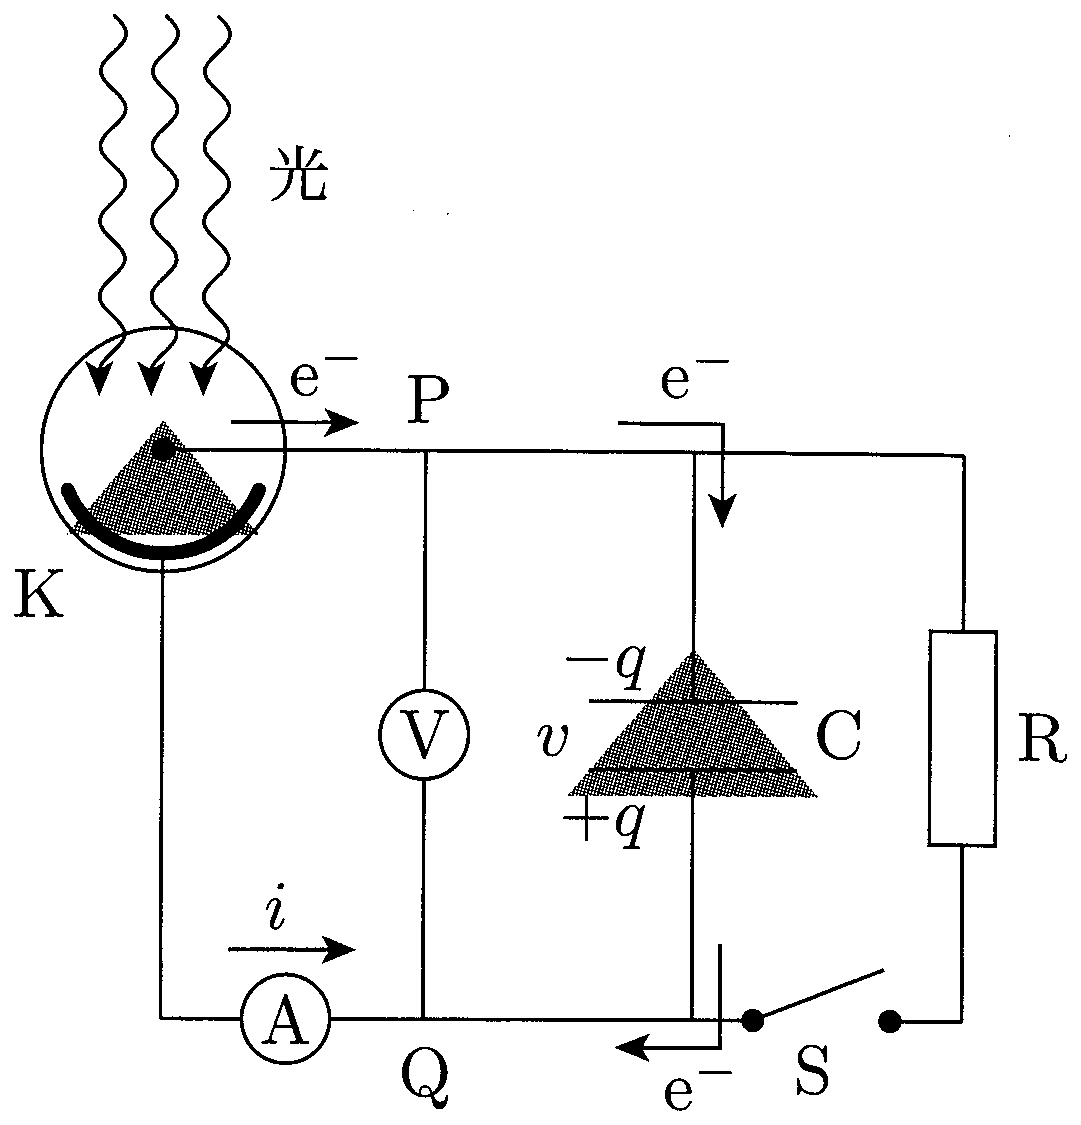
\includegraphics[keepaspectratio,width=40mm]{fig/n33_a8_zu.png}\end{center}
よって$v$，$i$は図のような向きであり，この光電管は，陽極に対する陰極の電圧$v$，および陰極から流れ出ていく電流$i$が図2のグラフに従う特性を持つ素子であると理解される．
\begin{komon}
\ko{1} 図2より，$v=1.8\U{V}$の電圧をかけたときに陰極$\mathrm{K}$から発せられた光電子が全く陽極にたどり着くことができなくなる．$\mathrm{K}$の仕事関数を$W$とすると
       \[\frac{hc}{\lambda_1}=K_{\max 1}+W\]
       また$v=1.8\U{V}$は阻止電圧であるから
       \[K_{\max 1}=e\times 1.8\fallingdotseq 2.9\times 10^{-19}\U{J}\Ans\]
\ko{2} 電子が陽極にたどり着いている間は回路に電流が流れてコンデンサー$\mathrm{C}$の帯電量が増加し，$\mathrm{C}$にかかる電圧$v$が増加していく．しかし，$\mathrm{C}$にかかる電圧が阻止電圧まで達するとついに回路には電流が流れなくなり，帯電量はそれ以上増加しなくなる．このとき$v=1.8\U{V}$であるから
       \[Q_0=C\times 1.8=9.0\times 10^{-6}\U{C}\Ans\]
\ko{3} 定常状態においてコンデンサーにかかっている電圧を$v$とすると，抵抗，光電管にも同じ電圧$v$がかかっている．このとき流れている電流$i$と$v$の間には図2の関係が成立している．
       \begin{center}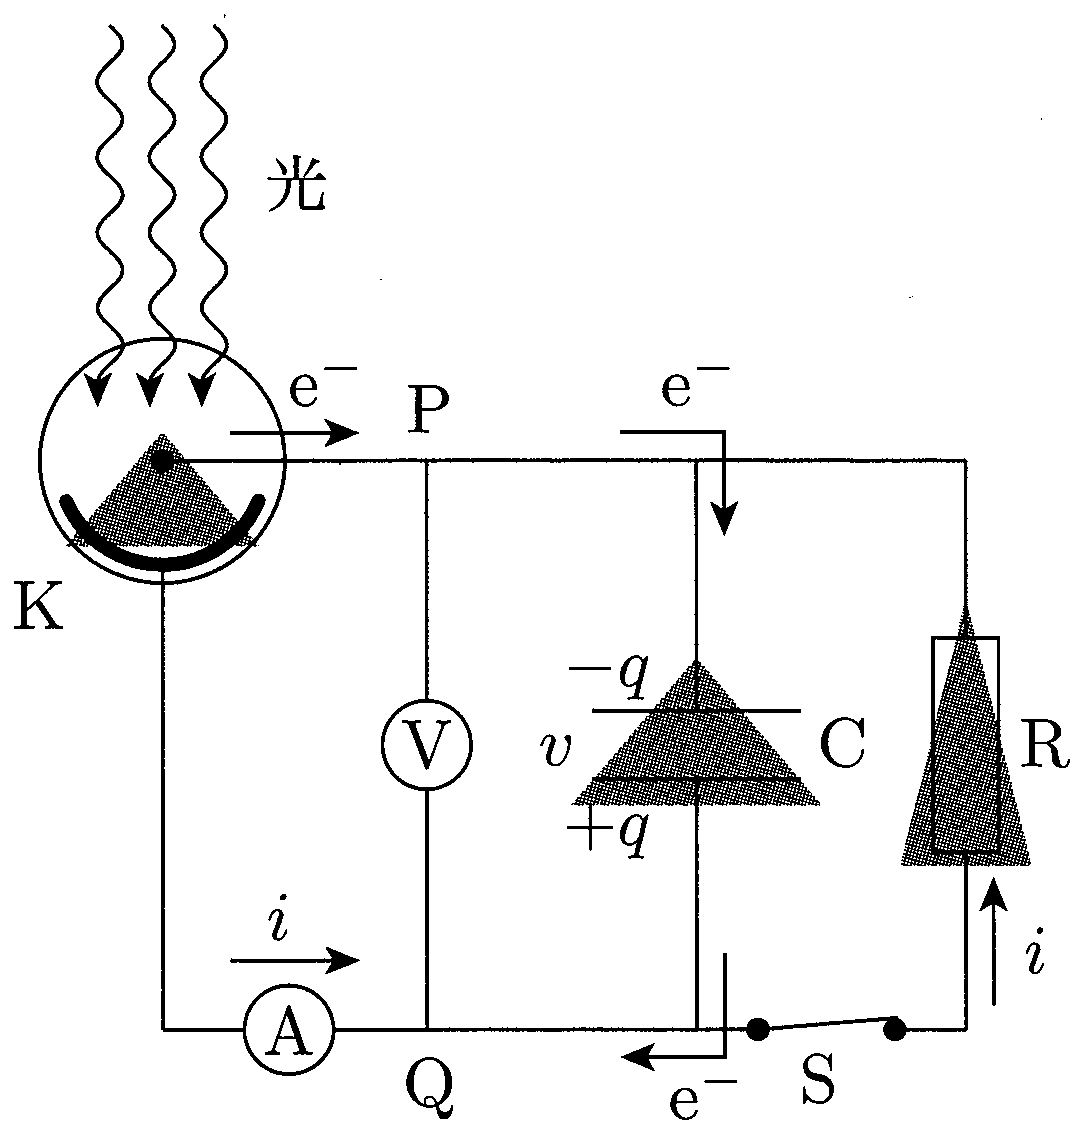
\includegraphics[keepaspectratio,width=40mm]{fig/n33_a8_zu2.png}\end{center}
       定常電流を$i_0$とすると，キルヒホッフの第二法則より$v=Ri_0$が成立するので，これを図2のグラフ中に記入して交点を取ると
       \begin{center}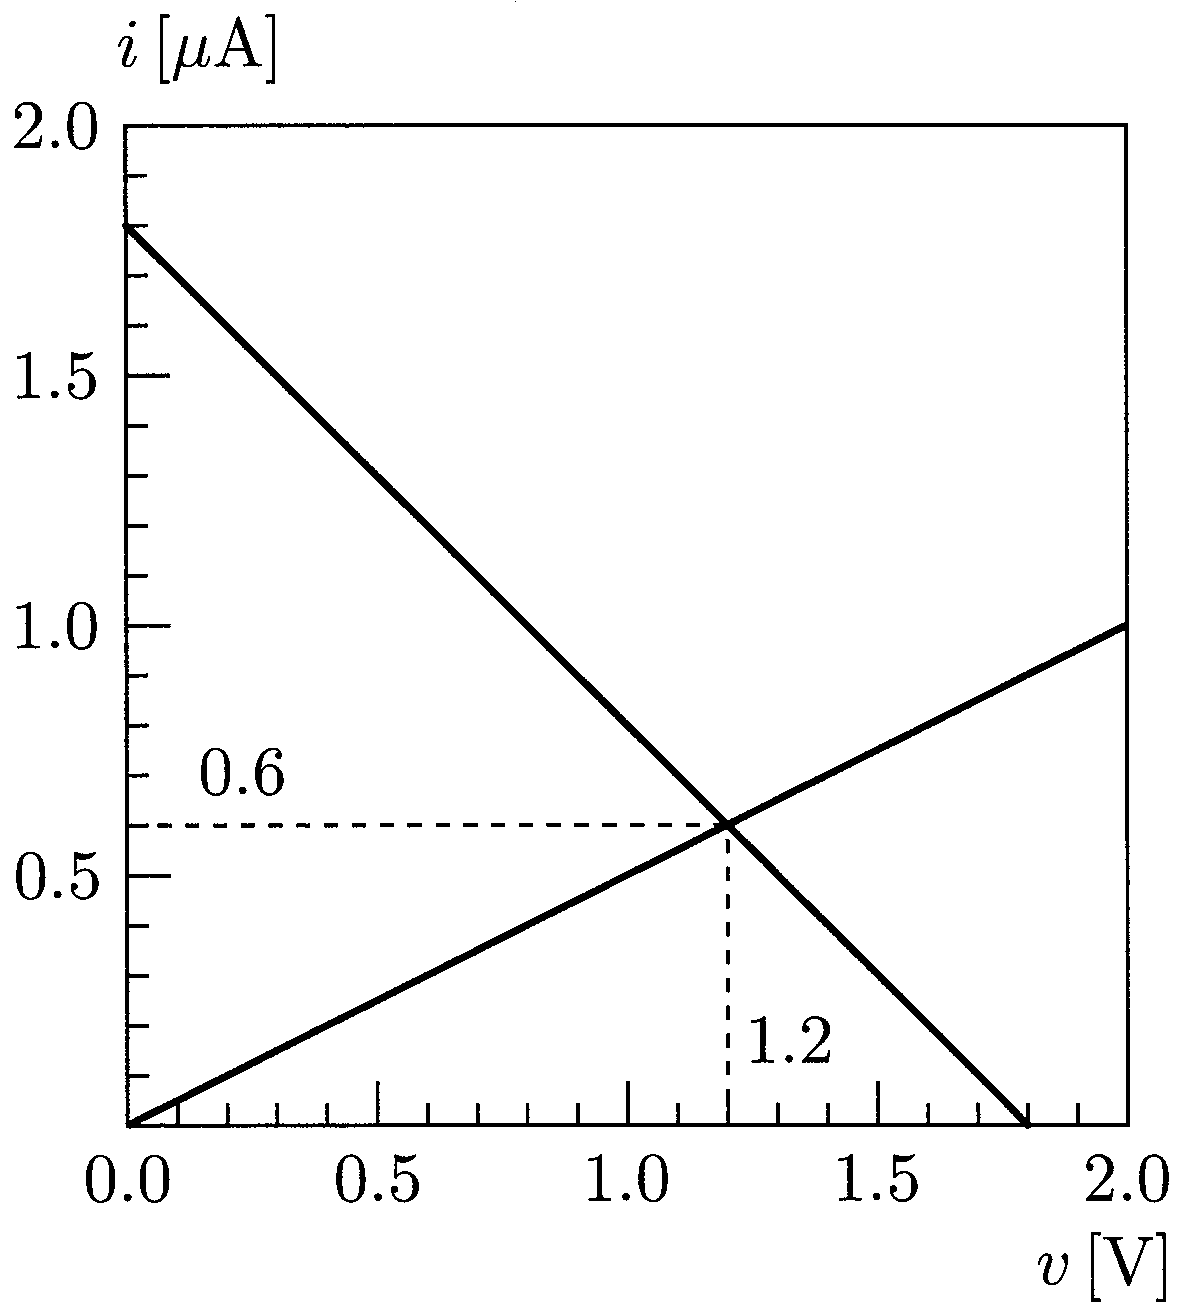
\includegraphics[keepaspectratio,width=44mm]{fig/n33_a8_graph.png}\end{center}
       \[i_0=0.6\U{\mu A}=6\times 10^{-7}\U{A}\Ans\]
\ko{4} (1)と同様に考えると，波長$\lambda_2$の光に対しての阻止電圧が$1.0\U{V}$であるから，$K_{\max 2}=e\times 1.0=1.6\times 10^{-19}\U{J}$であり，$\dfrac{hc}{\lambda_2}=K_{\max 2}+W$．(1)の式と合わせて$W$を消去すると
       \[h=\frac{K_{\max 1}-K_{\max 2}}{c\bigl(\frac{1}{\lambda_1}-\frac{1}{\lambda_2}\bigr)}\fallingdotseq 6.4\times 10^{-34}\U{J\cdot s}\]
       \hspace*{\fill}$\cdots$(答)
\end{komon}

\MonN{9}{フランク・ヘルツの実験}\par\nopagebreak
\begin{sisin}
有名なフランク・ヘルツの実験であるが，初見では何が起こっているのか分かりづらい難問であろう．(1)のヒントをよく読み取り，何が起きているのかを考えよう．大きな運動エネルギーを持つ電子が水銀原子に衝突した場合には水銀原子を励起し，その結果，励起に必要な分のエネルギー$E_2-E_1$を失う，ということに気付ければ簡単に攻められるはず．グラフが$4.9\U{V}$おきの繰り返しになっているのは，$E_2-E_1=4.9\U{eV}$であるためである．
% 原本は「E2−E1＝4.9[J]」（eV の誤り）．
なお，衝突の前後でエネルギーが保存される衝突を弾性衝突，またエネルギーが失われる衝突を非弾性衝突という（力学の反発係数を復習せよ）．
\end{sisin}
\KaiHead
\begin{komon}
\ko{1} ア：加速\qquad イ：弾性衝突\qquad ウ：$E_2-E_1$\qquad エ：非弾性衝突\qquad オ：減速\qquad カ：多い\qquad キ：大きい\Ans
\ko{2} ク：\MARU{3}\qquad ケ：\MARU{4}\qquad コ：\MARU{3}\Ans
\end{komon}

\end{multicols}
